%-----------------------------------------------------------------------------------------------------------%
\newpage

\setcounter{chapter}{3}
\setcounter{example}{0}
\setcounter{eqtn}{0}
\setcounter{section}{0}


\chapter{\lr{\textbf{تبدیل ها}}}
\textbf{\vspace{-140pt}}
\begin{figure}[H]
    \centering
    \setlength{\belowcaptionskip}{-10pt}
    
\includegraphics[width=0.8\textwidth]{Images/4/3/4.Session.1.3.0}
    \label{fig:4.Session.1.3.0}
\end{figure}
\textbf{\vspace{20pt}}
{
    \Large
    \begin{spacing}{1.5}
        ما اشیاء موجود در جهان های سه بعدی خود را به صورت هندسی توصیف می کنیم.
        یعنی به صورت مجموعه ای از مثلث هایی که با سطوح بیرونی اجسام تقریب دارند.
        اگر اشیاء ما بی حرکت بمانند، دنیای غیر جالبی خواهیم داشت.
        بنابراین ما به روش هایی برای تبدیل هندسی علاقه مند هستیم.
        نمونه‌هایی از تبدیل‌های هندسی عبارتند از: انتقال، دوران و مقیاس‌بندی.
        در این فصل، معادلات ماتریسی را توسعه می‌دهیم که می‌توان از آنها برای تبدیل نقاط و بردارها در فضای سه‌بعدی استفاده کرد.
        \\

        \textbf{\LARGE \hspace{-40pt}اهداف:}
        \begin{enumerate}[label=\textbf{\arabic*}.]
            \item {درک چگونگی نشان دادن تبدیل های خطی و وابسته با ماتریس ها.}
            \item {یادگیری تبدیل مختصات برای مقیاس بندی، دوران و انتقال هندسی.}
            \item {کشف چگونگی ترکیب کردن چندین ماتریس تبدیل به یک ماتریس تبدیل خالص از طریق ضرب ماتریس-ماتریس.}
            \item {فهمیدن چگونگی تبدیل سیستم مختصات به سیستم مختصات دیگر و چگونگی نشان دادن این تغییر تبدیل مختصات با یک ماتریس.}
            \item {آشنایی با زیر مجموعه توابع ارائه شده توسط کتابخانه ریاضی \lr{DirectX} که برای ساخت ماتریس های تبدیل استفاده می شوند.}
        \end{enumerate}
    \end{spacing}
}
%-----------------------------------------------------------------------------------------------------------%
\newpage

\setcounter{figure}{0}
\renewcommand{\thefigure}{\arabic{figure}.\arabic{chapter}}


\section{\textbf{تبدیلات خطی}}
\label{sec:3.1}
\subsection{\textbf{تعریف}}
{
    \Large
    \begin{spacing}{1.5}
        تابع ریاضی $\tau(\textbf{v})=\tau(x,y,z)=(x\prime,y\prime,z\prime)$ را در نظر بگیرید.
        این تابع یک بردار سه بعدی را دریافت کرده و یک بردار سه بعدی را خروجی می دهد.
        می گوییم که $\tau$ یک تبدیل خطی است اگر و تنها اگر که ویژگی های زیر برقرار باشد:

        \begin{eqtn}{eqtn:3.1}
            \centering
            $\tau(\textbf{u}+\textbf{v})=\tau(\textbf{u})\tau(\textbf{v})$\\
            $\tau(k\textbf{u})=k\tau(\textbf{u})$
        \end{eqtn}

        که در آن $\textbf{u}=(u_x,u_y,u_z)$ و $\textbf{v}=(v_x,v_y,v_z)$ بردار سه بعدی هستند و $k$ یک اسکالر است.

        \begin{point}{pnt:3.1}
            یک تبدیل خطی می تواند شامل مقادیر ورودی و خروجی غیر از بردارهای سه بعدی باشد،
            اما ما در کتاب گرافیک سه بعدی نیازی به چنین کلیتی نداریم.
        \end{point}

        \begin{example}{exp:3.1}
            \Large
            تابع $\tau(x,y,z)=(x^2,y^2,z^2)$ را تعریف کنید.
            به عنوان مثال، $\tau(1,2,3)=(1,3,9)$. این تابع خطی نیست زیرا برای $k=2$ و $\textbf{u}=(1,2,3)$، داریم:

            \begin{center}
                $\tau(k\textbf{u})=\tau(2,4,6)=(4,16,36)$
            \end{center}

            اما

            \begin{center}
                $k\tau(\textbf{u})=2(1,4,9)=(2,8,18)$
            \end{center}

            بنابراین خاصیت 2 معادله \ref{eqtn:3.1} برآورده نمی شود.
            اگر $\tau$ خطی باشد، نتیجه می شود که:

            \begin{eqtn}{eqtn:3.2}
                \centering
                \begin{equation*}
                    \centering
                    \begin{split}
                        \tau(a\textbf{u}+b\textbf{v}+c\textbf{w})&=\tau(a\textbf{u}+(b\textbf{v}+c\textbf{w})) \\
                        &=a\tau(\textbf{u})+\tau(b\textbf{v}+c\textbf{w})\\
                        &=a\tau(\textbf{u})+b\tau(\textbf{v})+c\tau(\textbf{w})
                    \end{split}
                \end{equation*}
            \end{eqtn}

            در بخش بعدی از این نتیجه استفاده خواهیم کرد.
        \end{example}
    \end{spacing}
}

\subsection{\textbf{نمایش ماتریسی}}
{
    \Large
    \begin{spacing}{1.5}
        فرض کنید $\textbf{u}=(x,y,z)$.
        همیشه می توانیم این را به صورت زیر بنویسیم:

        \begin{center}
            $\textbf{u}=(x,y,z)=x\textbf{i}+y\textbf{j}+z\textbf{k}=x(1,0,0)+y(0,1,0)+z(0,0,1)$
        \end{center}

        بردارهای $\textbf{i}=(1,0,0)$، $\textbf{j}=(0,1,0)$، و $\textbf{k}=(0,0,1)$، که بردارهای واحدی هستند
        که به ترتیب در امتداد محورهای مختصات کاری هدف قرار می گیرند، بردارهای پایه استاندارد برای $\mathbb{R}^3$ نامیده می شوند.
        ($\mathbb{R}^3$ مجموعه تمام بردارهای مختصات سه بعدی (x، y، z) را نشان می دهد).
        حال اجازه دهید $\tau$ یک تبدیل خطی باشد.
        با خطی بودن (یعنی معادله \ref{eqtn:3.2})، داریم:

        \begin{figure}[H]
            \centering
            \setlength{\belowcaptionskip}{-10pt}
            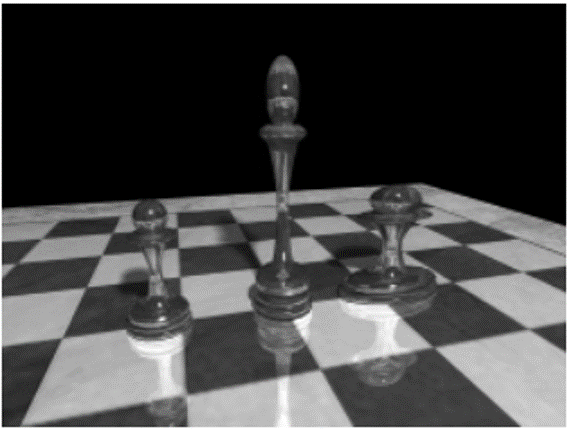
\includegraphics[width=0.5\textwidth]{Images/4/3/4.Session.1.3.1}
            \caption {سرباز سمت چپ شی اصلی است.
            سرباز میانی همان سرباز اصلی است که 2 واحد در محور y مقیاس دارد و آن را بلندتر می کند.
            سرباز سمت راست همان سرباز اصلی است که 2 واحد در محور x مقیاس دارد و آن را چاق تر می کند.}
            \label{fig:4.Session.1.3.1}
        \end{figure}

        \begin{eqtn}{eqtn:3.3}
            \centering
            $\tau(\textbf{u})=\tau(x\textbf{i}+y\textbf{j}+z\textbf{k})=x\tau(\textbf{i})+y\tau(\textbf{j})+z\tau(\textbf{k})$
        \end{eqtn}

        \begin{eqtn}{eqtn:3.4}
            \centering

            \begin{equation*}
                \centering
                \begin{split}
                    \tau(\textbf{u})&=x\tau(\textbf{i})+y\tau(\textbf{j})+z\tau(\textbf{k}) \\
                    &=\textbf{uA}=[x,y,z]\begin{bmatrix}
                                             \leftarrow & \tau(\textbf{i}) & \rightarrow \\
                                             \leftarrow & \tau(\textbf{j}) & \rightarrow \\
                                             \leftarrow & \tau(\textbf{k}) & \rightarrow
                    \end{bmatrix}=[x,y,z]\begin{bmatrix}
                                             A_{11} & A_{12} & A_{13} \\
                                             A_{21} & A_{22} & A_{23} \\
                                             A_{31} & A_{32} & A_{33}
                    \end{bmatrix}
                \end{split}
            \end{equation*}
        \end{eqtn}

        که در آن $\tau(\textbf{i})=(A_{11},A_{12},A_{13})$، $\tau(\textbf{j})=(A_{21},A_{22},A_{23})$، و $\tau(\textbf{k})=(A_{31},A_{32},A_{33})$.
        ماتریس $\textbf{A}$ را نمایش ماتریسی تبدیل خطی $\tau$ می نامیم.
    \end{spacing}
}

\subsection{\textbf{مقیاس بندی}}
{
    \Large
    \begin{spacing}{1.5}
        مقیاس بندی به تغییر اندازه یک شی اشاره دارد که در شکل \ref{fig:4.Session.1.3.1} نشان داده شده است.
        ما تحول مقیاس گذاری را توسط:

        \begin{center}
            $S(x,y,z)=(s_{x}x,s_{y}y,s_{z}z)$
        \end{center}

        این بردار را با واحدهای $s_x$ در محور $x$، واحدهای $s_y$ در محور $y$، و واحدهای $s_z$ در محور $z$،
        نسبت به مبدأ سیستم مختصات کار مقیاس بندی می‌کند.
        اکنون نشان می دهیم که $S$ در واقع یک تبدیل خطی است. ما داریم که:

        \begin{equation*}
            \centering
            \begin{split}
                S(\textbf{u}+\textbf{v})&=\left( s_{x}(u_{x}+v_{x}), s_{y}(u_{y}+v_{y}), s_{z}(u_{z}+v_{z}) \right) \\
                &=(s_{x}u_{x}+s_{x}v_{x}, s_{y}u_{y}+s_{y}v_{y}, s_{z}u_{z}+s_{z}v_{z}) \\
                &=(s_{x}u_{x}, s_{y}u_{y}, s_{z}u_{z})+(s_{x}v_{x}, s_{y}v_{y}, s_{z}v_{z}) \\
                &=S(\textbf{u})+S(\textbf{v}) \\
                S(k\textbf{u})&=(s_{x}ku_{x}, s_{y}ku_{y}, s_{z}ku_{z}) \\
                &=K(s_{x}u_{x}, s_{y}u_{y}, s_{z}u_{z}) \\
                &=KS(\textbf{u}) \\
            \end{split}
        \end{equation*}

        بنابراین هر دو ویژگی معادله \ref{eqtn:3.1} برآورده شدند، بنابراین $S$ خطی است،
        و بنابراین یک نمایش ماتریسی وجود دارد. برای یافتن نمایش ماتریس، ما فقط $S$ را به هر یک از بردارهای پایه استاندارد، مانند رابطه \ref{eqtn:3.3} اعمال می کنیم،
        و سپس بردارهای حاصل را در ردیف های یک ماتریس قرار می دهیم (مانند معادله \ref{eqtn:3.4}):

        \begin{center}
            $S(\textbf{i})=(s_x\cdot 1,s_y\cdot 0,s_z\cdot 0)=(s_x,0,0) \\
            S(\textbf{j})=(s_x\cdot 0,s_y\cdot 1,s_z\cdot 0)=(0,s_y,0) \\
            S(\textbf{k})=(s_x\cdot 0,s_y\cdot 0,s_z\cdot 1)=(0,0,s_z)$
        \end{center}

        بنابراین نمایش ماتریسی $S$ به صورت زیر است:

        \begin{center}
            $\textbf{S}=\begin{bmatrix}
                            s_x & 0   & 0   \\
                            0   & s_y & 0   \\
                            0   & 0   & s_z
            \end{bmatrix}$
        \end{center}

        ما این ماتریس را ماتریس مقیاس بندی می نامیم.
        معکوس ماتریس مقیاس بندی به صورت زیر بدست می آید:

        \begin{center}
            $\textbf{S}^{-1}=\begin{bmatrix}
                                 1/s_x & 0     & 0     \\
                                 0     & 1/s_y & 0     \\
                                 0     & 0     & 1/s_z
            \end{bmatrix}$
        \end{center}

        \begin{example}{exp:3.2}
            \Large
            فرض کنید مربعی داریم که با یک نقطه حداقل $(-4,-4, 0)$ و یک نقطه حداکثر $(4,4,0)$ تعریف شده است.
            اکنون فرض کنید که می خواهیم مربع را $0.5$ واحد در محور $x$، $2.0$ واحد در محور $y$، و محور $z$ را بدون تغییر رها کنیم.
            ماتریس مقیاس بندی مربوطه به صورت زیر است:

            \begin{center}
                $\textbf{S}=\begin{bmatrix}
                                0.5 & 0 & 0 \\
                                0   & 2 & 0 \\
                                0   & 0 & 1
                \end{bmatrix}$
            \end{center}

            \begin{figure}[H]
                \centering
                \setlength{\belowcaptionskip}{-10pt}
                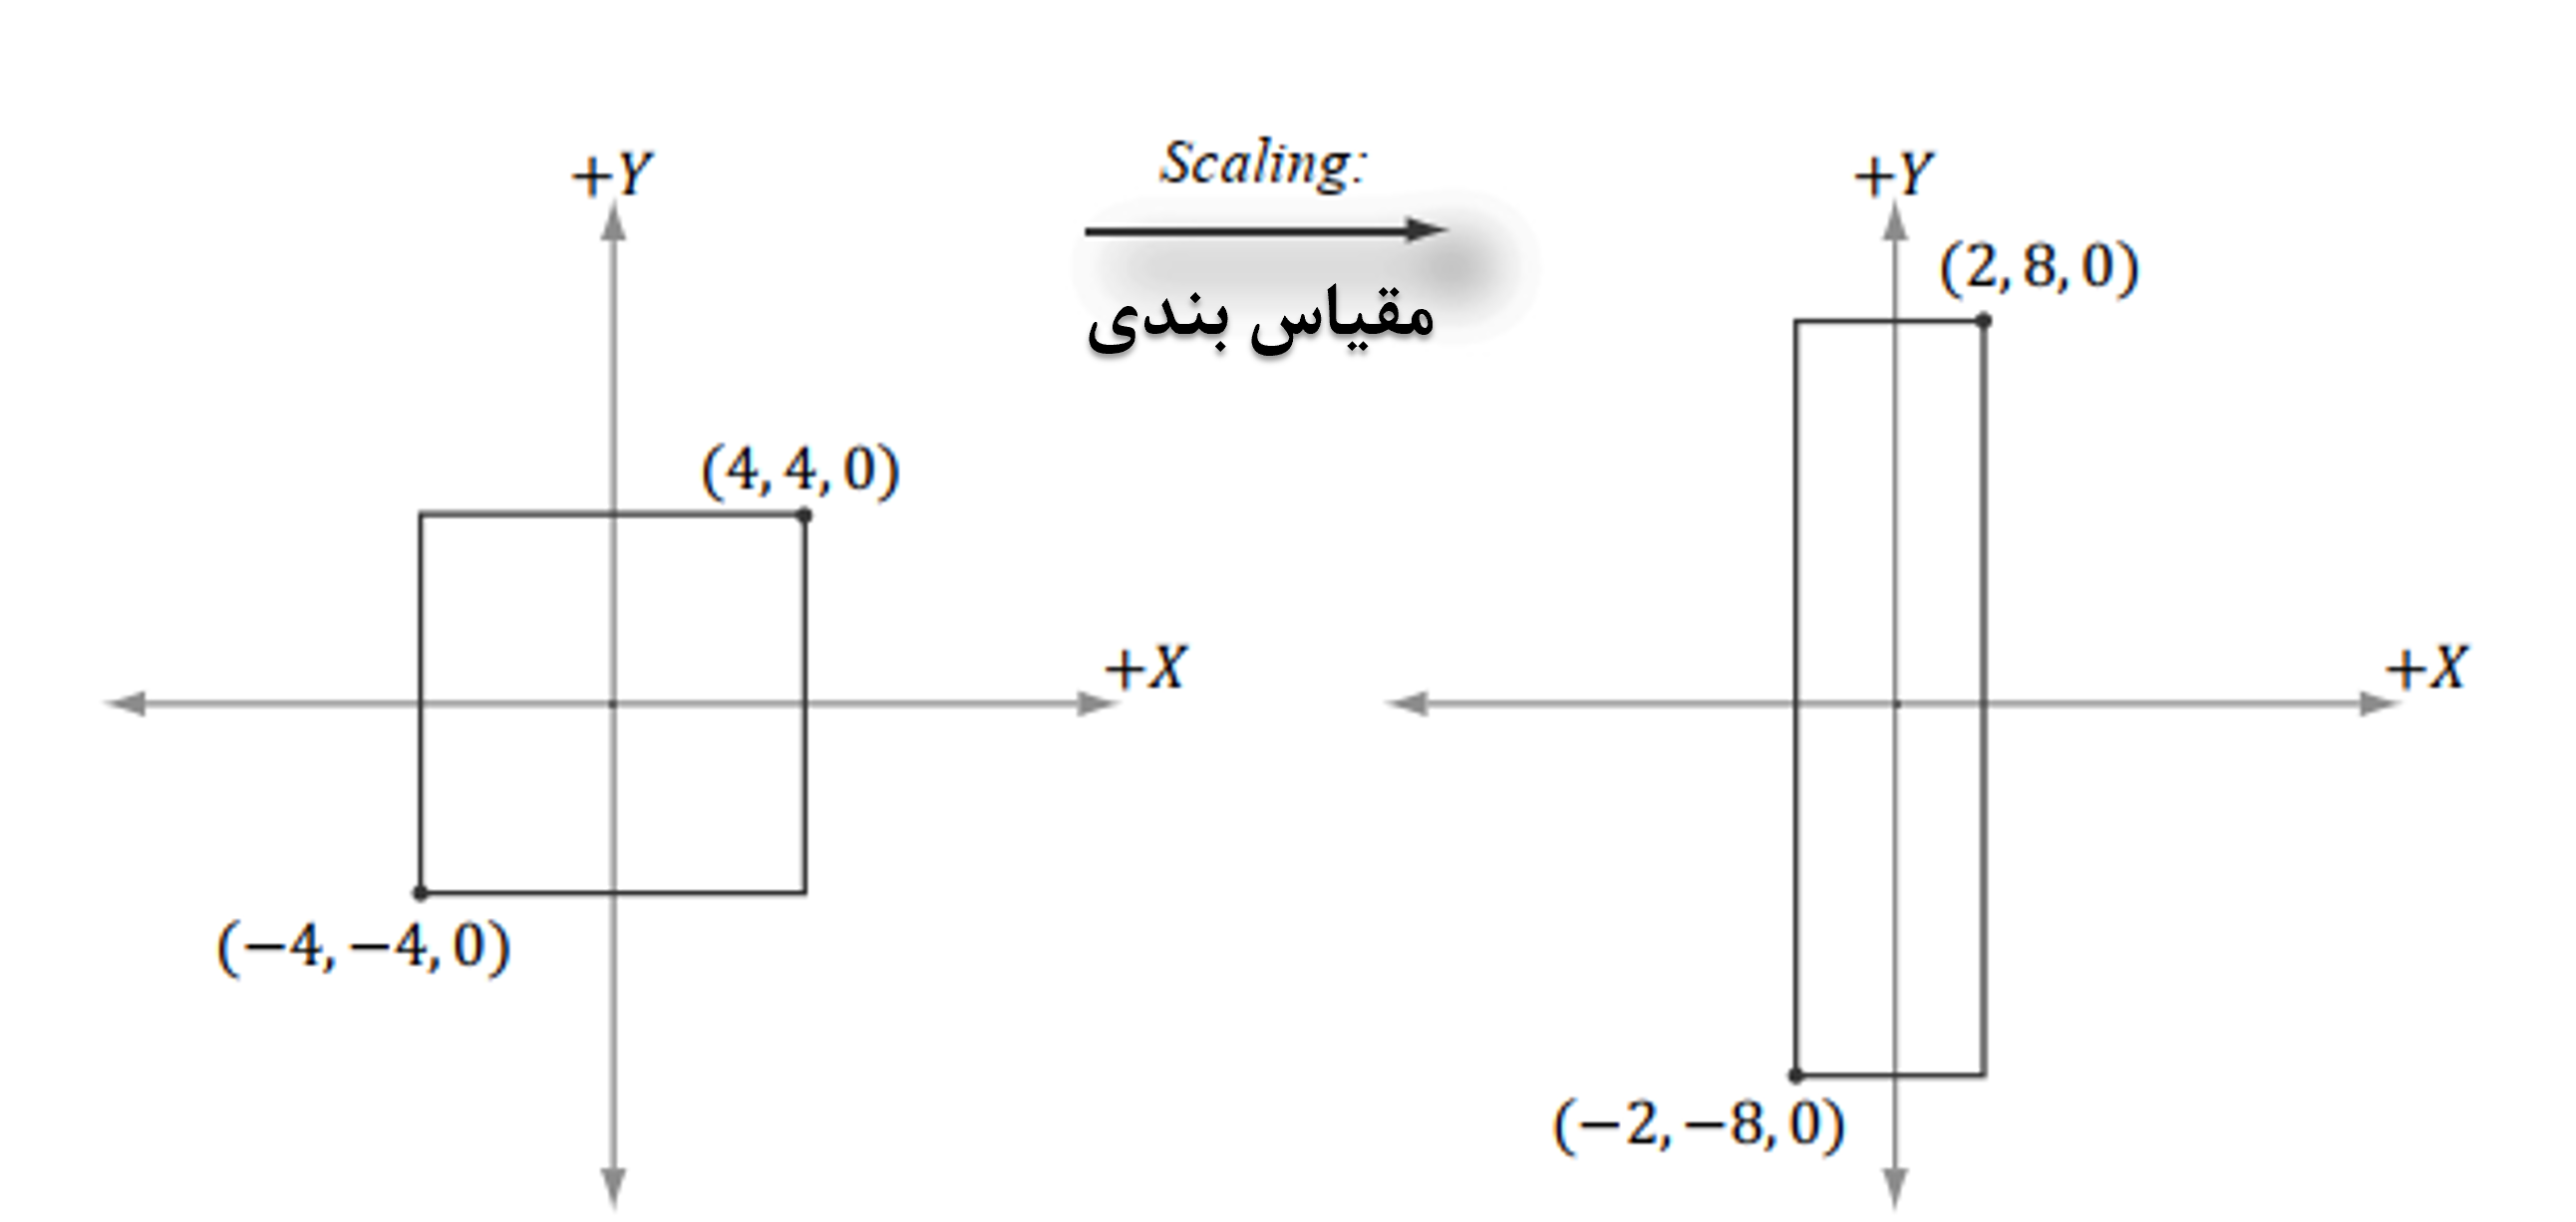
\includegraphics[width=0.8\textwidth]{Images/4/3/4.Session.1.3.2}
                \caption {مقیاس بندی به نیم واحد در محور x و دو واحد در محور y. توجه داشته باشید که هنگام نگاه کردن به محور z منفی، هندسه 2 بعدی است زیرا z=0 است.}
                \label{fig:4.Session.1.3.2}
            \end{figure}

            اکنون برای مقیاس (تبدیل) مربع، هر دو نقطه حداقل و حداکثر را در این ماتریس ضرب می کنیم:

            \begin{center}
                $[-4,-4,0]\begin{bmatrix}
                              0.5 & 0 & 0 \\
                              0   & 2 & 0 \\
                              0   & 0 & 1
                \end{bmatrix}=[-2,-8,0]$\hspace{5 mm}$[4,4,0]=\begin{bmatrix}
                                                                  0.5 & 0 & 0 \\
                                                                  0   & 2 & 0 \\
                                                                  0   & 0 & 1
                \end{bmatrix}=[2,8,0]$
            \end{center}

            نتیجه در شکل \ref{fig:4.Session.1.3.2} نشان داده شده است.
        \end{example}
    \end{spacing}
}

\subsection{\textbf{دوران}}
{
    \Large
    \begin{spacing}{1.5}
        در این بخش، دوران بردار $\textbf{v}$ حول محور $\textbf{n}$ با زاویه $\theta$ را شرح می دهیم.
        شکل \ref{fig:4.Session.1.3.3} را ببینید.
        توجه داشته باشید که هنگام نگاه کردن به محور $\textbf{n}$ زاویه را در جهت عقربه های ساعت اندازه می گیریم.
        علاوه بر این، فرض می کنیم $\norm{\textbf{n}}=1$.

        \begin{figure}[H]
            \centering
            \setlength{\belowcaptionskip}{-10pt}
            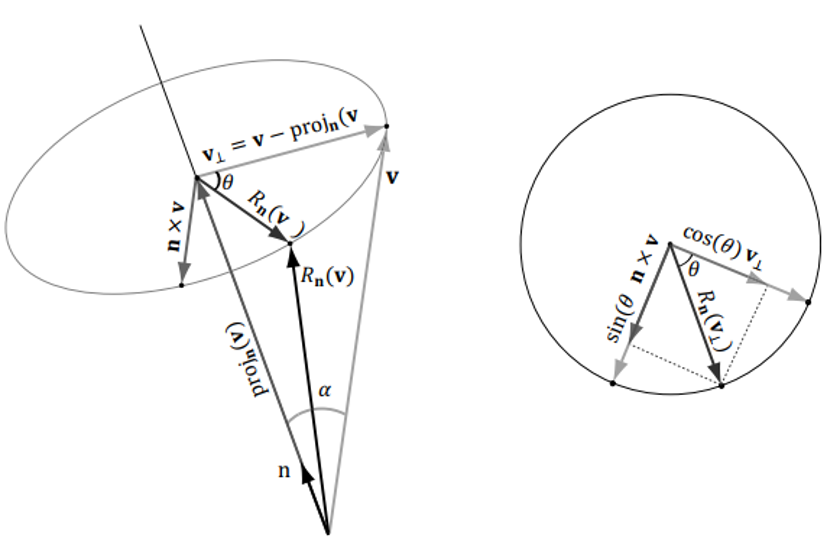
\includegraphics[width=0.8\textwidth]{Images/4/3/4.Session.1.3.3}
            \caption {هندسه دوران حول بردار $\textbf{n}$.}
            \label{fig:4.Session.1.3.3}
        \end{figure}

        ابتدا $\textbf{v}$ را به دو قسمت تجزیه کنید:
        یک قسمت موازی با $\textbf{n}$ و قسمت دیگر متعامد با $\textbf{n}$.
        قسمت موازی فقط projn(v) است (مثال \ref{exp:1.5} را به خاطر بیاورید).
        قسمت متعامد با $\textbf{v}_{\perp}=perp_{n}(\textbf{v})=\textbf{v}-proj_{n}(\textbf{v})$ داده می شود.
        (همچنین از مثال \ref{exp:1.5} به یاد بیاورید که از آنجایی که $\textbf{n}$ یک بردار واحد است، ما $proj_{n}(\textbf{v})= (\textbf{n}\cdot\textbf{v})\textbf{n}$ را داریم.)
        مشاهدات کلیدی این است که بخشی $proj_{n}(\textbf{v})$ که موازی با $\textbf{n}$ است ، تحت دوران ثابت است.
        بنابراین ما فقط باید بفهمیم که چگونه قسمت متعامد را دوران دهیم. یعنی بردار چرخشی $R_{n}(\textbf{v})=proj_{n}(\textbf{v})+R_{n}(\textbf{v}_{\perp})$، در شکل \ref{fig:4.Session.1.3.3}.
        برای یافتن $R_{n}(\textbf{v}_{\perp})$، یک سیستم مختصات دوبعدی را در صفحه دوران تنظیم کردیم.
        ما از $\textbf{v}_{\perp}$ به عنوان یک بردار مرجع استفاده خواهیم کرد.
        برای به دست آوردن یک بردار مرجع دوم متعامد به $\textbf{v}_{\perp}$ و $\textbf{n}$،
        حاصل ضرب متقاطع $\textbf{n}\times\textbf{v}$ (قانون شست دست چپ) را می گیریم. از مثلثات شکل \ref{fig:4.Session.1.3.3} و تمرین \ref{question14} از فصل 1، می بینیم که

        \begin{center}
            $\norm{\textbf{n}\times\textbf{v}}=\norm{\textbf{n}}\norm{\textbf{v}}\sin\alpha=\norm{\textbf{v}}\sin\alpha=\norm{\textbf{v}_{\perp}}$
        \end{center}

        که در آن $\alpha$ زاویه بین $\textbf{n}$ و $\textbf{n}$ است.
        بنابراین هر دو بردار مرجع دارای طول یکسانی هستند و روی دایره دوران قرار می گیرند.
        اکنون که این دو بردار مرجع را تنظیم کردیم، از مثلثات می بینیم که:

        \begin{center}
            $R_{n}(\textbf{v}_{\perp})=\cos\theta\textbf{v}_{\perp}+sin\theta(\textbf{n}\times\textbf{v})$
        \end{center}

        این فرمول دوران زیر را به ما می دهد:

        \begin{eqtn}{eqtn:3.5}
            \centering
            \begin{equation*}
                \centering
                \begin{split}
                    R_{n}(\textbf{v})&=proj_{n}(\textbf{v})+R_{n}(\textbf{v}_{\perp})\\
                    &=(\textbf{n}\cdot\textbf{v})\textbf{n}+\cos\theta\textbf{v}_{\perp}+\sin\theta(\textbf{n}\times\textbf{v})\\
                    &=(\textbf{n}\cdot\textbf{v})\textbf{n}+\cos\theta(\textbf{v}-(\textbf{n}\cdot\textbf{v})\textbf{n})+\sin\theta(\textbf{n}\times\textbf{v})\\
                    &=\cos\theta\textbf{v}+(1-\cos\theta)(\textbf{n}\cdot\textbf{v})\textbf{n}+\sin\theta(\textbf{n}\times\textbf{v})
                \end{split}
            \end{equation*}
        \end{eqtn}

        ما آن را به عنوان تمرینی رها می کنیم تا نشان دهیم که این یک تبدیل خطی است.
        برای یافتن نمایش ماتریس، ما فقط $R_{n}$ را به هر یک از بردارهای پایه استاندارد مانند معادله \ref{eqtn:3.3} اعمال می کنیم و سپس بردارهای حاصل را در ردیف های یک ماتریس قرار می دهیم (مانند معادله \ref{eqtn:3.4}).
        نتیجه نهایی این است:

        \begin{center}
            $\textbf{R}_{n}=\begin{bmatrix}
                                c+(1-c)x^{2} & (1-c)xy+sz   & (1-c)xz-sy \\
                                (1-c)xy-sz   & c+(1-c)y^{2} & (1-c)yz+sx \\
                                (1-c)xz+sy   & (1-c)yz-sx   & c+(1-c)z^{2}
            \end{bmatrix}$
        \end{center}

        جایی که $c=\cos\theta$ و $s=\sin\theta$ را فرض میکنیم.
        ماتریس های دوران خاصیت جالبی دارند. هر بردار ردیف واحد طول (تأیید) و بردارهای ردیف متعامد (تأیید) هستند.
        بنابراین بردارهای ردیف متعامد هستند (یعنی متعامد متعامد و طول واحد).
        به ماتریسی که ردیف‌های آن متعامد هستند، ماتریس متعامد گفته می‌شود.
        یک ماتریس متعامد دارای خاصیت جذابی است که معکوس آن در واقع برابر با جابجایی آن است. بنابراین، معکوس $R_{n}$ برابر است با:

        \begin{center}
            $\textbf{R}^{-1}_{n}=\textbf{R}^{T}_{n}=\begin{bmatrix}
                                                        c+(1-c)x^{2} & (1-c)xy-sz   & (1-c)xz+sy \\
                                                        (1-c)xy+sz   & c+(1-c)y^{2} & (1-c)yz-sx \\
                                                        (1-c)xz-sy   & (1-c)yz+sx   & c+(1-c)z^{2}
            \end{bmatrix}$
        \end{center}

        به طور کلی، ماتریس های متعامد برای کار با آنها مطلوب هستند، زیرا معکوس آنها برای محاسبه آسان و کارآمد است.
        به ویژه، اگر محورهای $x$، $y$ و $z$ را برای چرخش انتخاب کنیم (یعنی به ترتیب $\textbf{n}=(1,0,0)$، $\textbf{n}=(0,1,0)$ و $\textbf{n}=(0,0,1)$)،
        سپس ماتریس های دوران زیر را دریافت می کنیم که به ترتیب حول محور $x$، $y$ و $z$ دوران میکنند:

        \begin{center}
            $\textbf{R}_{x}=\begin{bmatrix}
                                1 & 0           & 0          & 0 \\
                                0 & \cos\theta  & \sin\theta & 0 \\
                                0 & -\sin\theta & \cos\theta & 0 \\
                                0 & 0           & 0          & 1
            \end{bmatrix}, \textbf{R}_{y}=\begin{bmatrix}
                                              \cos\theta & 0 & -\sin\theta & 0 \\
                                              0          & 1 & 0           & 0 \\
                                              \sin\theta & 0 & \cos\theta  & 0 \\
                                              0          & 0 & 0           & 1
            \end{bmatrix}, \textbf{R}_{z}=\begin{bmatrix}
                                              \cos\theta  & \sin\theta & 0 & 0 \\
                                              -\sin\theta & \cos\theta & 0 & 0 \\
                                              0           & 0          & 1 & 0 \\
                                              0           & 0          & 0 & 1
            \end{bmatrix}$
        \end{center}

        \begin{example}{exp:3.3}
            \Large
            فرض کنید مربعی داریم که با یک نقطه حداقل $(-1, 0, -1)$ و یک نقطه حداکثر $(1, 0, 1)$ تعریف شده است.
            حال فرض کنید که می‌خواهیم مربع $-30^\circ$ را در جهت عقربه‌های ساعت حول محور $y$ دوران دهیم (یعنی $30^\circ$ خلاف جهت عقربه‌های ساعت).
            در این مورد، $\textbf{n}=(0,1,0)$، که $\textbf{R}_{n}$ را به طور قابل توجهی ساده می کند.
            ماتریس دوران محور $y$  مربوطه به صورت زیر است:

            \begin{center}
                $\textbf{R}_{y}=\begin{bmatrix}
                                    \cos\theta & 0 & -\sin\theta \\
                                    0          & 1 & 0           \\
                                    \sin\theta & 0 & \cos\theta
                \end{bmatrix}=\begin{bmatrix}
                                  \cos(-30^\circ) & 0 & -\sin(-30^\circ) \\
                                  0               & 1 & 0                \\
                                  \sin(-30^\circ) & 0 & \cos(-30^\circ)
                \end{bmatrix}=\begin{bmatrix}
                                  \frac{\displaystyle \sqrt{\displaystyle 3}}{\displaystyle 2} & 0 & \frac{\displaystyle 1}{\displaystyle 2}                      \\
                                  0                                                            & 1 & 0                                                            \\
                                  \frac{\displaystyle 1}{\displaystyle 2}                      & 0 & \frac{\displaystyle \sqrt{\displaystyle 3}}{\displaystyle 2}
                \end{bmatrix}$
            \end{center}

            اکنون برای دوران (تبدیل) مربع، هر دو نقطه حداقل و حداکثر را در این ماتریس ضرب می کنیم:

            \begin{center}
                $[-1,0,-1]\begin{bmatrix}
                              \frac{\displaystyle \sqrt{\displaystyle 3}}{\displaystyle 2} & 0 & \frac{\displaystyle 1}{\displaystyle 2}                      \\
                              0                                                            & 1 & 0                                                            \\
                              \frac{\displaystyle 1}{\displaystyle 2}                      & 0 & \frac{\displaystyle \sqrt{\displaystyle 3}}{\displaystyle 2}
                \end{bmatrix}\approx[-0.36,0,-1.36]\hspace{5 mm}[1,0,1]\begin{bmatrix}
                                                                           \frac{\displaystyle \sqrt{\displaystyle 3}}{\displaystyle 2} & 0 & \frac{\displaystyle 1}{\displaystyle 2}                      \\
                                                                           0                                                            & 1 & 0                                                            \\
                                                                           \frac{\displaystyle 1}{\displaystyle 2}                      & 0 & \frac{\displaystyle \sqrt{\displaystyle 3}}{\displaystyle 2}
                \end{bmatrix}\approx[0.36,0,1.36]$
            \end{center}

            نتیجه در شکل \ref{fig:4.Session.1.3.4} نشان داده شده است.

            \begin{figure}[H]
                \centering
                \setlength{\belowcaptionskip}{-10pt}
                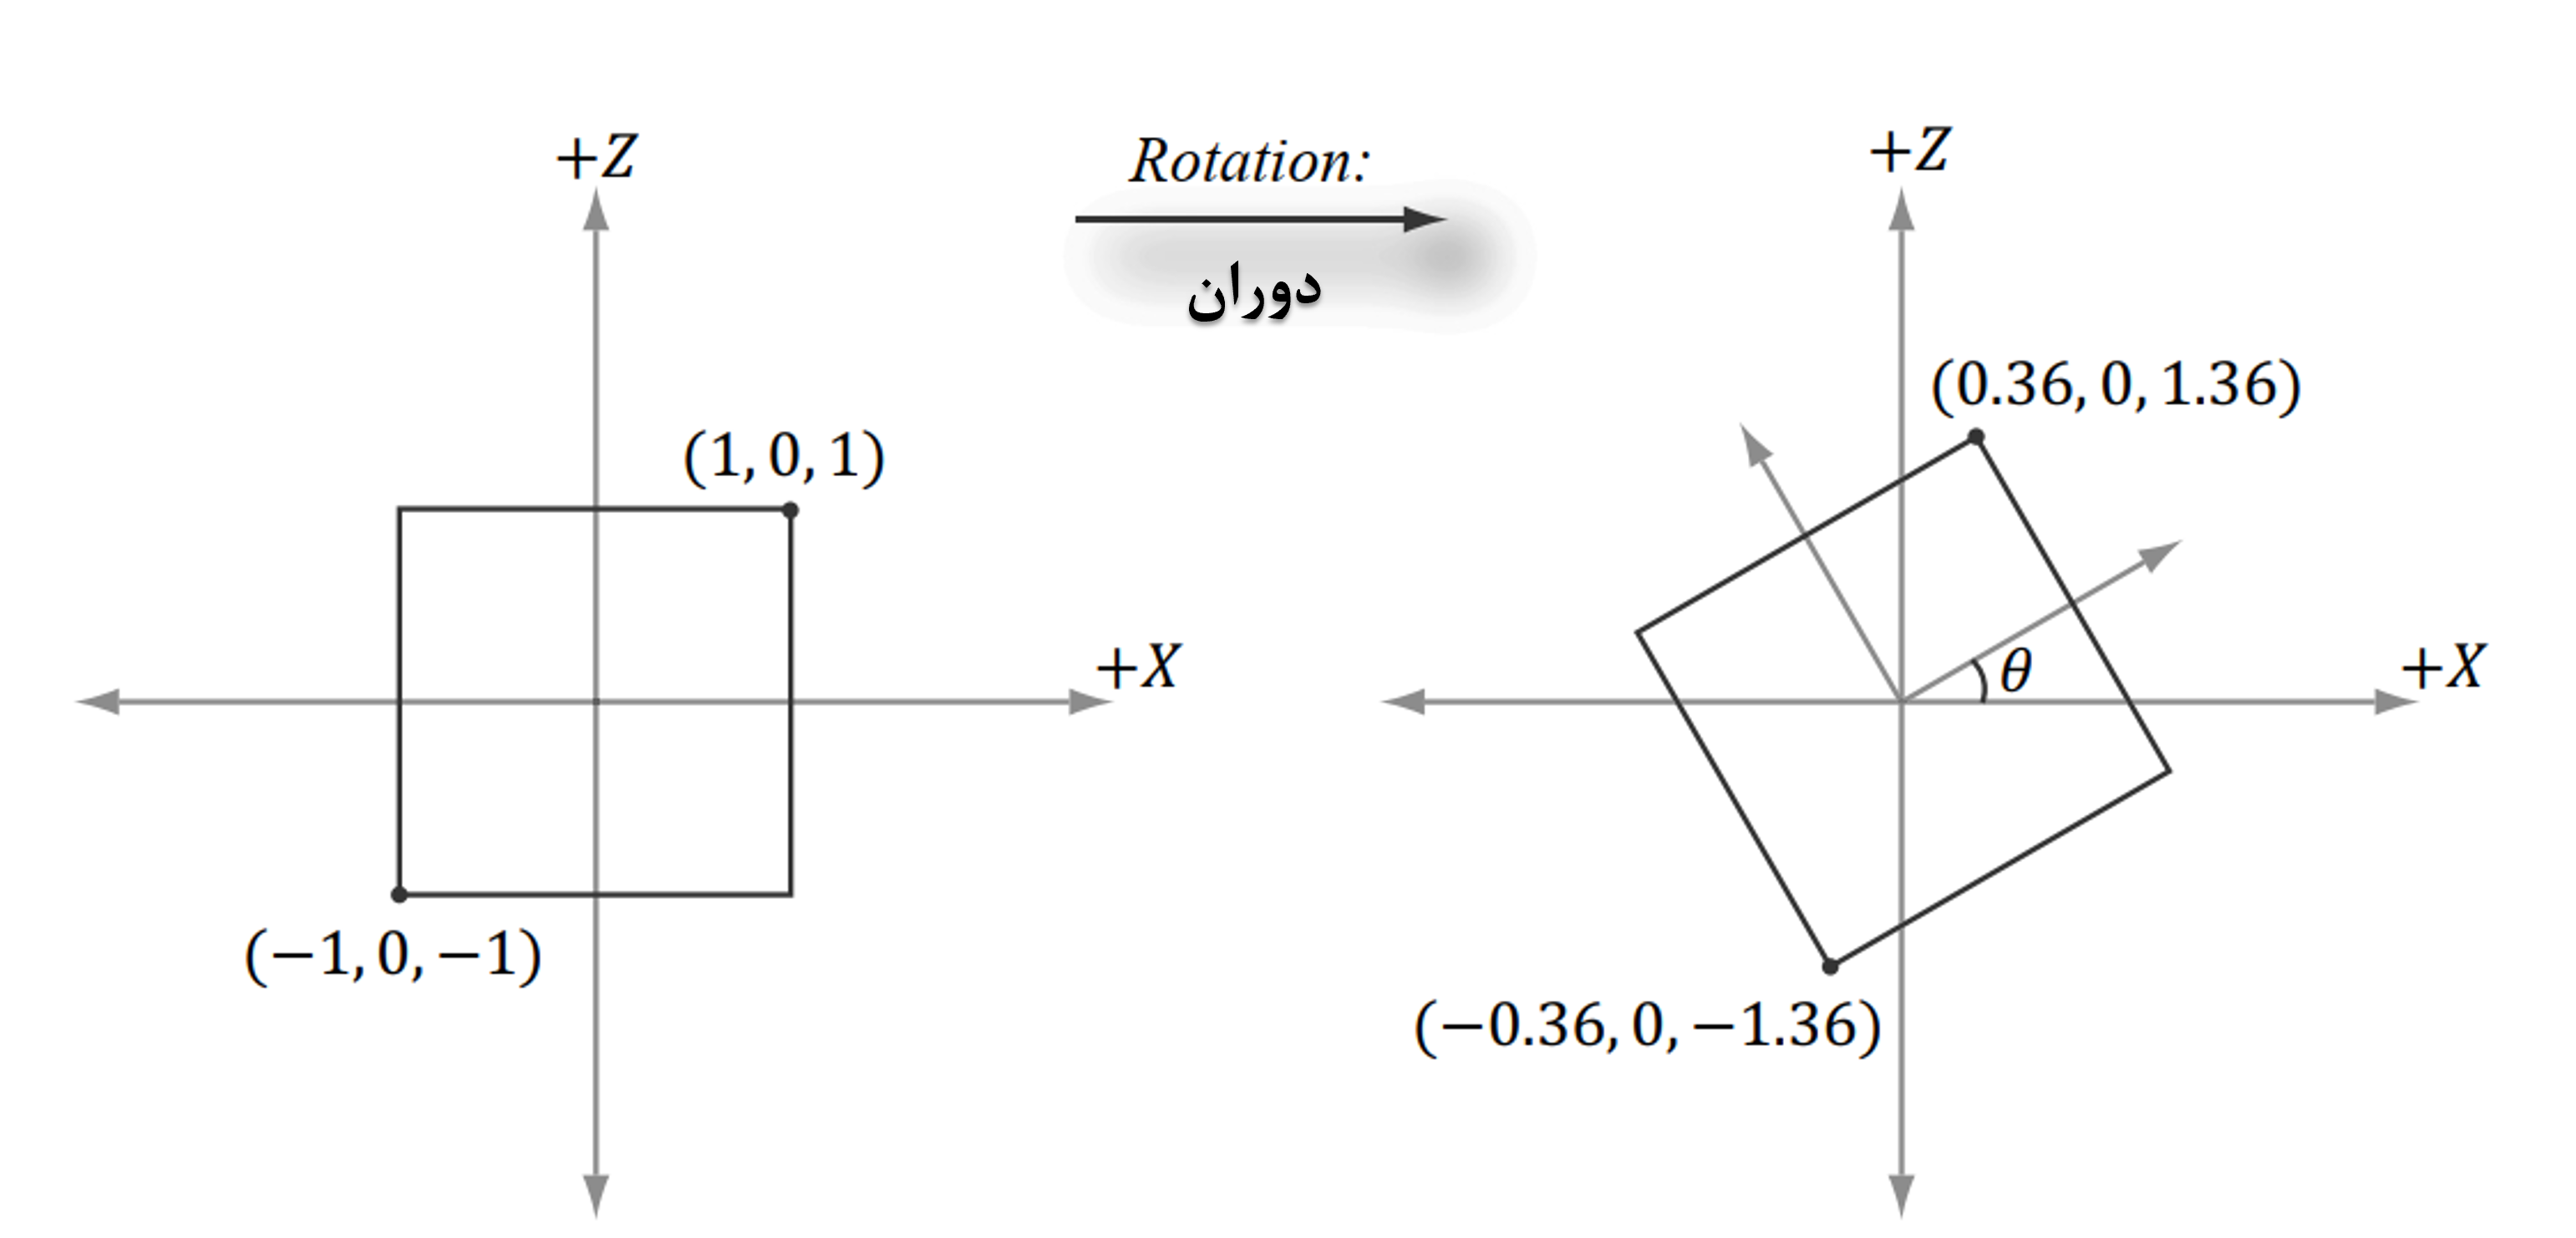
\includegraphics[width=0.8\textwidth]{Images/4/3/4.Session.1.3.4}
                \caption {دوران $-30^\circ$ در جهت عقربه های ساعت حول محور $y$.
                توجه داشته باشید که هنگام نگاه کردن به محور مثبت $y$، هندسه اساساً 2 بعدی است زیرا $y=0$ است.}
                \label{fig:4.Session.1.3.4}
            \end{figure}
        \end{example}
    \end{spacing}
}


\section{\textbf{تبدیلات آفین}}
\label{sec:3.2}
\subsection{\textbf{مختصات همگن}}
{
    \Large
    در بخش بعدی خواهیم دید که تبدیل آفین یک تبدیل خطی همراه با انتقال است.
    با این حال، انتقال برای بردارها معنی ندارد زیرا یک بردار فقط جهت و اندازه را، مستقل از مکان، توصیف می کند.
    به عبارت دیگر، بردارها باید تحت انتقال بدون تغییر باشند.
    انتقال ها فقط باید برای نقاط (به عنوان مثال، بردارهای موقعیت) اعمال شوند.
مختصات همگن مکانیسم نمادگذاری مناسبی را فراهم می کند که ما را قادر می سازد نقاط و بردارها را به طور یکنواخت مدیریت کنیم.
با مختصات همگن، ما به تاپل $4$ تایی منتقل میشویم و آنچه را که در چهارمین مختصات $w$ قرار می دهیم بستگی به این دارد که یک نقطه یا بردار را توصیف کنیم.
به طور خاص می نویسیم:
    \begin{spacing}{1.5}
        \lr{
            \begin{enumerate}[label=\textbf{\arabic*}.]
                \item {(x,y,z,0) \rl{برای بردار ها}}
                \item {(x,y,z,1) \rl{برای نقطه ها}}
            \end{enumerate}
        }

        بعداً خواهیم دید که تنظیم $w=1$ برای نقاط به انتقال نقاط اجازه می دهد تا به درستی کار کنند
        و تنظیم $w=0$  برای بردارها از تغییر مختصات بردارها توسط انتقال ها جلوگیری می کند
        (ما نمی خواهیم مختصات یک بردار را انتقال دهیم که جهت و بزرگی آن را تغییر دهد - انتقال ها نباید خواص بردارها را تغییر دهند).

        \begin{point}{pnt:3.1}
            \Large
            علامت گذاری مختصات همگن با ایده های نشان داده شده در شکل \label{fig:4.Session.1.1.17} مطابقت دارد.
            یعنی تفاوت بین دو نقطه $\textbf{q-p}=(q_{x},q_{y},q_{z},1)\textbf{-}(p_{x},p_{y},p_{z},1)=(q_{x}-p_{x},q_{y}-p_{y},q_{z}-p_{z},0)$ منجر به بردار،
            و یک نقطه به اضافه یک بردار $\textbf{p+v}=(q_{x},q_{y},q_{z},1)\textbf{+}(v_{x},v_{y},v_{z},1)=(q_{x}+v_{x},q_{y}+v_{y},q_{z}+v_{z},1)$ منجر به نقطه میشود.
        \end{point}
    \end{spacing}
}

\subsection{\textbf{تعریف و نمایش ماتریس}}
{
    \Large
    \begin{spacing}{1.5}
        یک تبدیل خطی نمی تواند تمام تبدیل هایی را که ما می خواهیم انجام دهیم را توصیف کند.
        بنابراین، ما به یک کلاس بزرگتر از توابع به نام تبدیل های آفین تقویت میکنیم.
        تبدیل آفین یک تبدیل خطی به اضافه یک بردار انتقال $\textbf{b}$ است. به این معنا که:

        \begin{center}
            $\alpha(\textbf{u})=\tau(\textbf{u})+\textbf{b}$
        \end{center}

        یا در نماد ماتریسی:

        \begin{center}
            $\alpha(\textbf{u})=\textbf{uA}+\textbf{b}=[x, y, z]\begin{bmatrix}
                                                                    A_{11} & A_{12} & A_{13} \\
                                                                    A_{21} & A_{22} & A_{23} \\
                                                                    A_{31} & A_{32} & A_{33}
            \end{bmatrix}+[b_{x},b_{y},b_{z}]=[x\prime,y\prime,z\prime]$
        \end{center}

        که در آن $\textbf{A}$ نمایش ماتریسی یک تبدیل خطی است.

        اگر مختصات همگن را با $w=1$ افزایش دهیم، می‌توانیم این را فشرده‌تر بنویسیم:

        \begin{eqtn}{eqtn:3.6}
            \centering
            $[x, y, z, 1]\begin{bmatrix}
                             A_{11} & A_{12} & A_{13} & 0 \\
                             A_{21} & A_{22} & A_{23} & 0 \\
                             A_{31} & A_{32} & A_{33} & 0
                             b_{x} & b_{y} & b_{y} & 1
            \end{bmatrix}=[x\prime, y\prime, z\prime,1]$
        \end{eqtn}

        ماتریس $4\times 4$ در معادله \ref{eqtn:3.6} نمایش ماتریسی تبدیل آفین نامیده می شود.
        توجه کنید که جمع با $\textbf{b}$ اساساً یک انتقال است (یعنی تغییر در موقعیت).
        ما نمی خواهیم این را برای بردارها اعمال کنیم زیرا بردارها موقعیتی ندارند.
        با این حال، ما هنوز هم می خواهیم قسمت خطی تبدیل آفین را به بردارها اعمال کنیم.
        اگر $w=1$ را در جزء چهارم برای بردارها قرار دهیم، انتقال $\textbf{b}$ اعمال نمی شود (با انجام ضرب ماتریس بررسی کنید).

        \begin{point}{pnt:3.1}
            \Large
            از آنجا که ضرب داخلی بردار ردیف با ستون چهارم ماتریس تبدیل آفین $4\times 4$ فوق ، برابر است با:
            $[x, y, z, w]\cdot[0,0,0,1]=w$، این ماتریس مختصات $w$ بردار ورودی را تغییر نمی دهد.
        \end{point}
    \end{spacing}
}

\subsection{\textbf{انتقال}}
{
    \Large
    \begin{spacing}{1.5}
        تبدیل همانی یک تبدیل خطی است که فقط آرگومان خود را برمی‌گرداند.
        یعنی $I\textbf{u}=\textbf{u}$.
        می توان نشان داد که نمایش ماتریسی این تبدیل خطی، ماتریس همانی است.

        حال، تبدیل انتقال را به صورت تبدیل آفین تعریف می کنیم که تبدیل خطی آن تبدیل همانی است. به این معنا که،

        \begin{center}
            $\tau(\textbf{u})=\textbf{uI}+\textbf{b}=\textbf{u}+\textbf{b}$
        \end{center}

        \begin{figure}[H]
            \centering
            \setlength{\belowcaptionskip}{-10pt}
            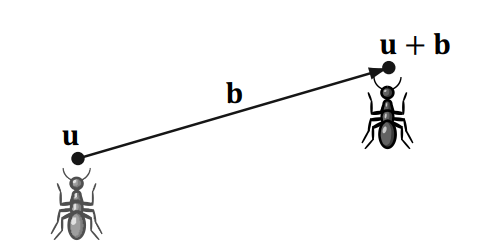
\includegraphics[width=0.5\textwidth]{Images/4/3/4.Session.1.3.5}
            \caption {جابجایی موقعیت مورچه با مقدار بردار جابجایی $\textbf{b}$.}
            \label{fig:4.Session.1.3.5}
        \end{figure}

        همانطور که می بینید، این به سادگی نقطه $\textbf{u}$ را با $\textbf{b}$ انتقال میدهد (یا جابجا می کند).
        شکل \ref{fig:4.Session.1.3.5} نشان می دهد که چگونه می توان از آن برای جابجایی اشیا استفاده کرد - ما هر نقطه روی شی را با همان بردار $\textbf{b}$ انتقال میدهیم تا آن را جابجا کنیم.
        با معادله \ref{eqtn:3.6}، $\tau$ نمایش ماتریسی زیر را دارد:

        \begin{center}
            $\textbf{T}=\begin{bmatrix}
                            1 & 0 & 0 & 0 \\
                            0 & 1 & 0 & 0 \\
                            0 & 0 & 1 & 0
                            b_{x} & b_{y} & b_{y} & 1
            \end{bmatrix}$
        \end{center}

        به این ماتریس انتقال می گویند.

        معکوس ماتریس انتقال به صورت زیر بدست می آید:

        \begin{center}
            $\textbf{T}^{-1}=\begin{bmatrix}
                                 1 & 0 & 0 & 0 \\
                                 0 & 1 & 0 & 0 \\
                                 0 & 0 & 1 & 0
                                 -b_{x} & -b_{y} & -b_{y} & 1
            \end{bmatrix}$
        \end{center}

        \begin{example}{exp:3.4}
            \Large
            فرض کنید مربعی داریم که با یک نقطه حداقل $(-8, 2, 0)$ و یک نقطه حداکثر $(-2, 8, 0)$ تعریف شده است.
            اکنون فرض کنید که می‌خواهیم مربع را $12$ واحد در محور $x$، $-10$ واحد در محور $y$ انتقال دهیم
            و محور $z$ را بدون تغییر رها کنیم.
            ماتریس انتقال مربوطه به صورت زیر است:

            \begin{center}
                $\textbf{T}^{-1}=\begin{bmatrix}
                                     1 & 0 & 0 & 0 \\
                                     0 & 1 & 0 & 0 \\
                                     0 & 0 & 1 & 0
                                     12 & -10 & 0 & 1
                \end{bmatrix}$
            \end{center}

            اکنون برای انتقال (تبدیل) مربع، هر دو نقطه حداقل و حداکثر را در این ماتریس ضرب می کنیم:

            \begin{center}
                $[-8, 2, 0, 1]\begin{bmatrix}
                                  1 & 0 & 0 & 0 \\
                                  0 & 1 & 0 & 0 \\
                                  0 & 0 & 1 & 0
                                  12 & -10 & 0 & 1
                \end{bmatrix}=[4, -8, 0, 1]$ \\
                $[-2, 8, 0, 1]\begin{bmatrix}
                                  1 & 0 & 0 & 0 \\
                                  0 & 1 & 0 & 0 \\
                                  0 & 0 & 1 & 0
                                  12 & -10 & 0 & 1
                \end{bmatrix}=[10, -2, 0, 1]$
            \end{center}

            نتیجه در شکل \ref{fig:4.Session.1.3.6} نشان داده شده است.

            \begin{figure}[H]
                \centering
                \setlength{\belowcaptionskip}{-10pt}
                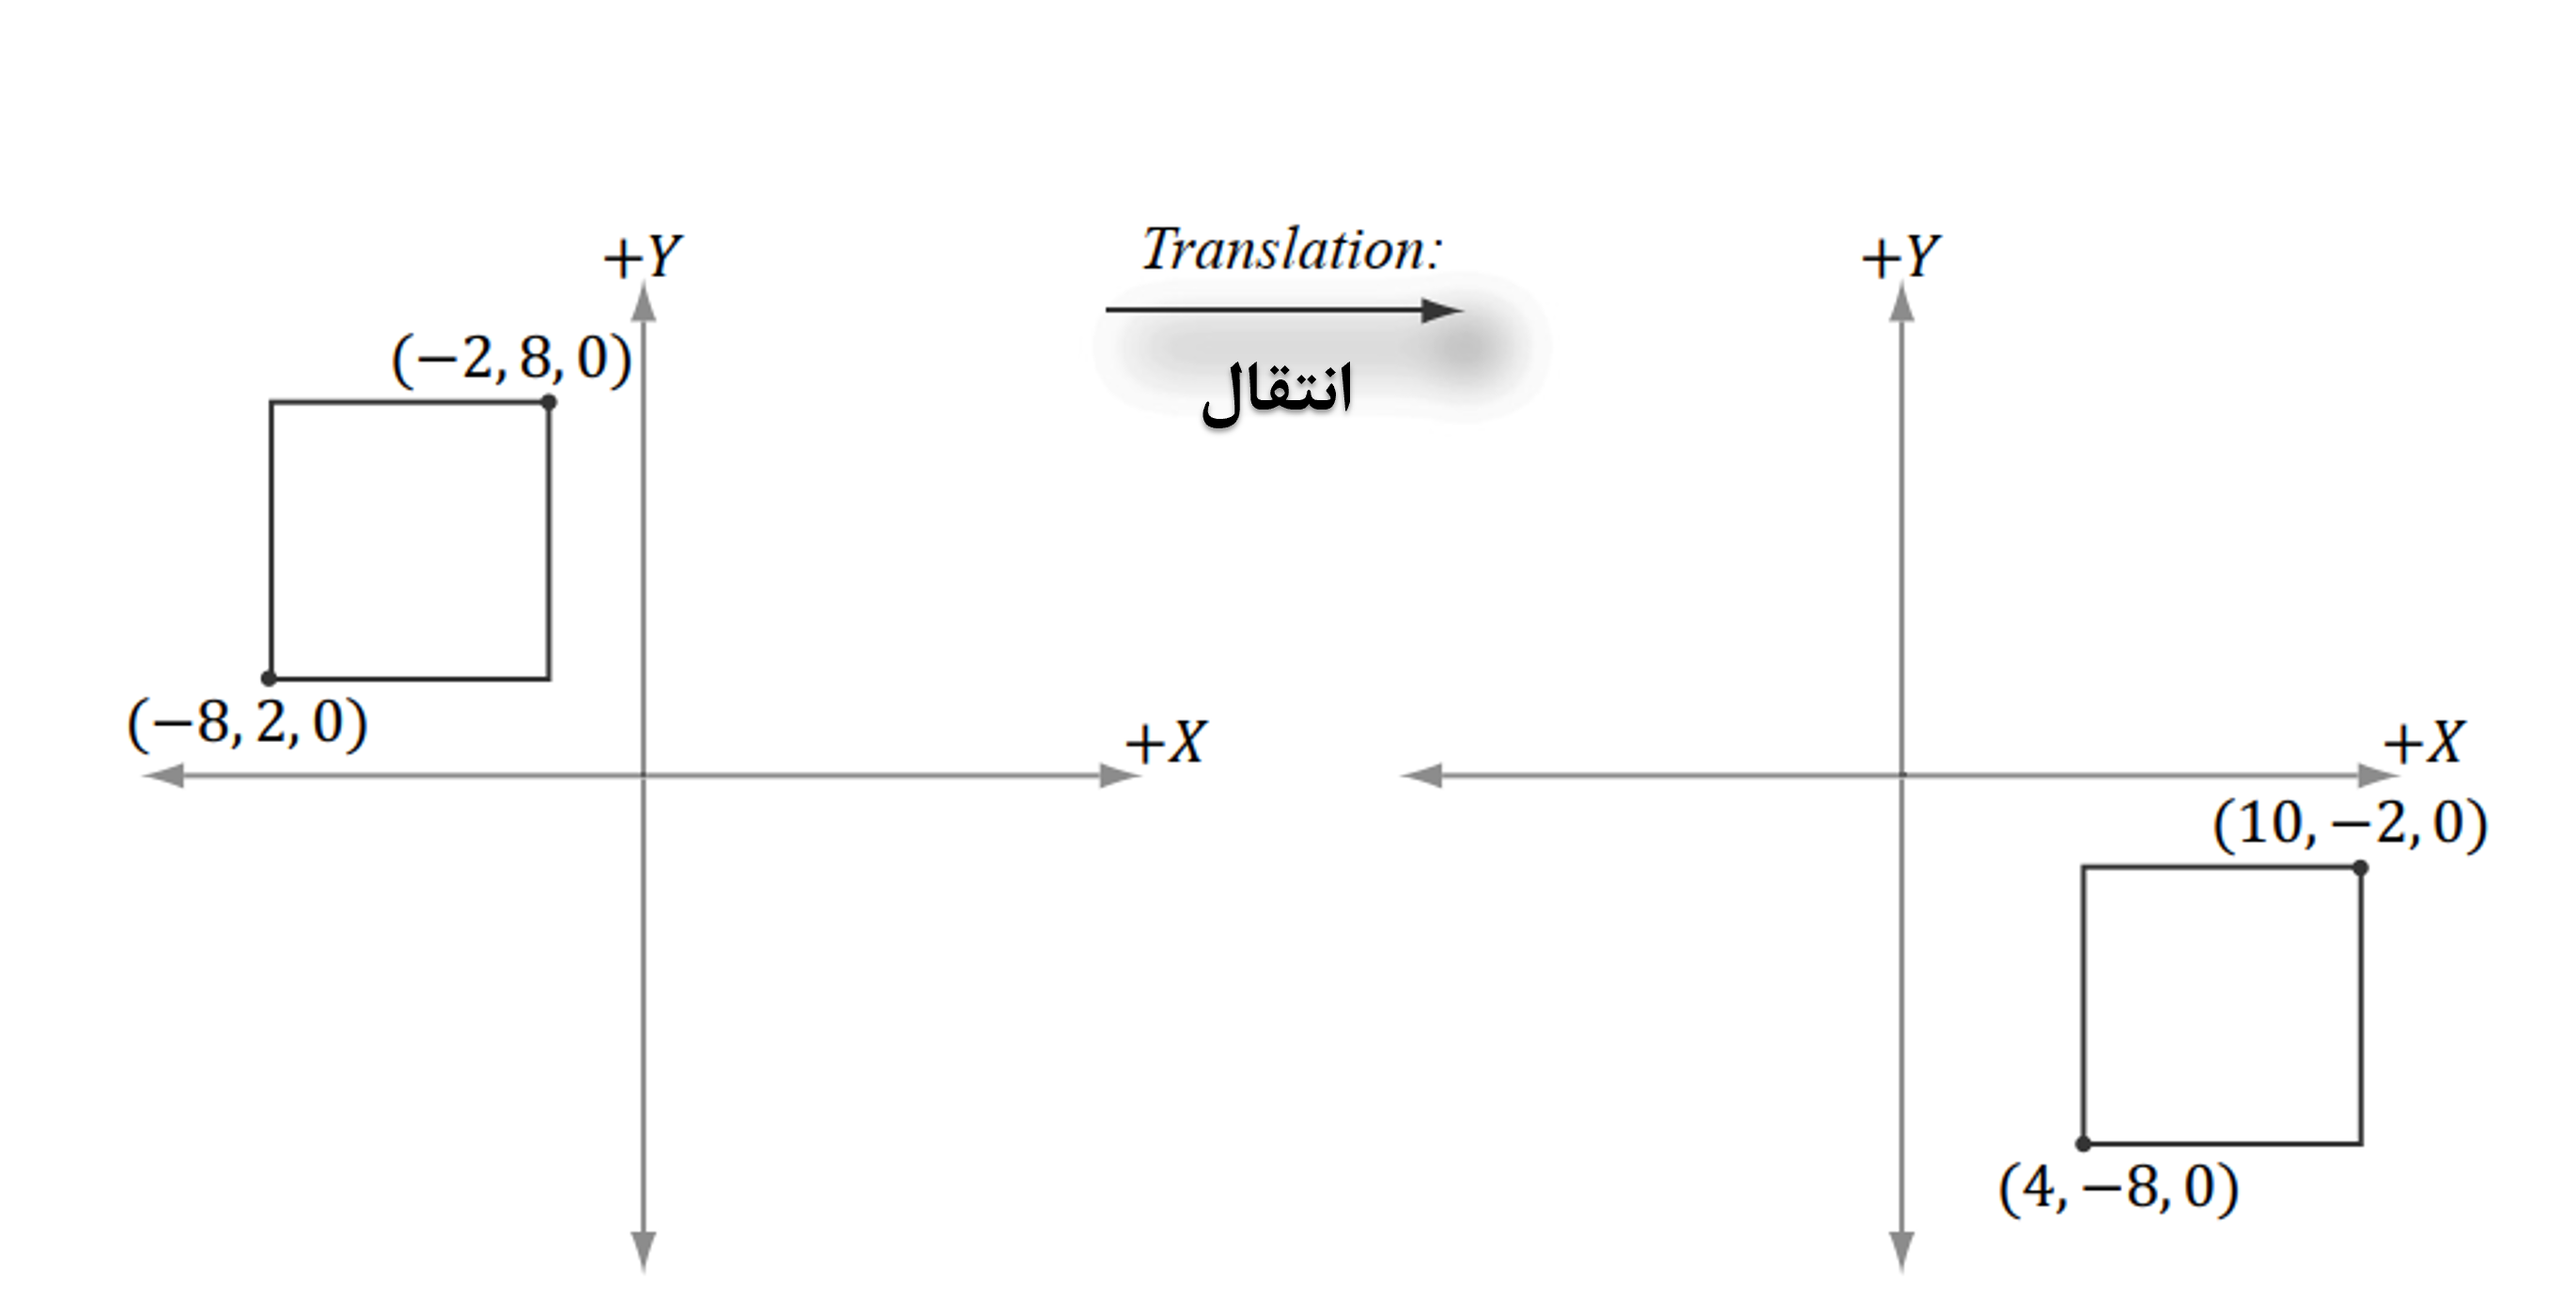
\includegraphics[width=0.8\textwidth]{Images/4/3/4.Session.1.3.6}
                \caption {انتقال $12$ واحد در محور $x$ و $-10$ واحد در محور $y$.
                توجه داشته باشید که هنگام نگاه کردن به محور $z$ منفی، هندسه اساساً 2 بعدی است زیرا $z=0$ است.}
                \label{fig:4.Session.1.3.6}
            \end{figure}
        \end{example}

        \begin{point}{pnt:3.1}
            \Large
            بگذارید $\textbf{T}$ یک ماتریس تبدیل باشد و به یاد بیاورید که با محاسبه حاصلضرب $\textbf{vT=v\prime}$ یک نقطه/بردار را تبدیل می کنیم.
            توجه کنید که اگر یک نقطه/بردار را با $\textbf{T}$ تبدیل کنیم و سپس دوباره آن را با $\textbf{T}^{-1}$ معکوس تبدیل کنیم،
            به بردار اصلی می‌رسیم: $\textbf{vTT^{-1}=vI=v}$.
            به عبارت دیگر، تبدیل معکوس ، تبدیل را خنثی می کند.
            به عنوان مثال، اگر یک نقطه را $5$ واحد در محور $x$ انتقال داده، و سپس برعکس $-5$ واحد در محور $x$ انتقال دهیم، به جایی می رسیم که شروع کرده ایم.
            به همین ترتیب، اگر نقطه ای را $30^\circ$ درجه حول محور $y$ دوران دهیم، و سپس برعکس $-30^\circ$ درجه حول محور $y$ دوران دهیم، در نهایت به نقطه اصلی خود می رسیم.
            به طور خلاصه، معکوس یک ماتریس تبدیل، تبدیل مخالف را انجام می دهد، به طوری که ترکیب دو تبدیل، هندسه را بدون تغییر می گذارد.
        \end{point}
    \end{spacing}
}

\subsection{\textbf{ماتریس های وابسته برای مقیاس بندی و دوران}}
{
    \Large
    \begin{spacing}{1.5}
        مشاهده کنید که اگر $\textbf{b}=0$ باشد، تبدیل آفین به تبدیل خطی کاهش می یابد.
        بنابراین ما می‌توانیم هر تبدیل خطی را به‌عنوان یک تبدیل آفین با $\textbf{b}=0$ بیان کنیم.
        این به نوبه خود به این معنی است که می‌توانیم هر تبدیل خطی را با یک ماتریس آفین $4\times 4$ نشان دهیم.
        به عنوان مثال، ماتریس های مقیاس بندی و دوران نوشته شده با استفاده از ماتریس $4\times 4$ به صورت زیر آورده شده است:

        \begin{center}
            $\textbf{S}=\begin{bmatrix}
                            s_x & 0   & 0   & 0 \\
                            0   & s_y & 0   & 0 \\
                            0   & 0   & s_z & 0 \\
                            0   & 0   & 0   & 1
            \end{bmatrix}$ \\
            \begin{bmatrix}
                c+(1-c)x^{2} & (1-c)xy+sz & (1-c)xz-sy & 0\\
                (1-c)xy-sz & c+(1-c)y^{2} & (1-c)yz+sx & 0\\
                (1-c)xz+sy & (1-c)yz-sx & c+(1-c)z^{2} & 0
                0 & 0 & 0 & 1
            \end{bmatrix}
        \end{center}

        به این ترتیب، می‌توانیم تمام تبدیل‌های خود را با استفاده از ماتریس $4\times 4$ و نقطه و بردار با استفاده از بردار ردیف همگن $4\times 1$ بیان کنیم.
    \end{spacing}
}

\subsection{\textbf{تفسیر هندسی یک ماتریس تبدیل وابسته}}
{
    \Large
    \begin{spacing}{1.5}
        در این بخش، شهودی از معنای هندسی اعداد درون ماتریس تبدیل آفین ایجاد می کنیم.
        ابتدا، اجازه دهید یک تبدیل جسم صلب را در نظر بگیریم، که اساساً یک تبدیل حفظ شکل است.
        یک مثال در دنیای واقعی از تبدیل جسم صلب ممکن است برداشتن یک کتاب از روی میز و قرار دادن آن در قفسه کتاب باشد.
        در طول این فرآیند شما کتاب را از روی میز خود به قفسه کتاب انتقال میدهید، اما به احتمال زیاد جهت کتاب را در فرآیند (دوران) تغییر می دهید.
        فرض کنید $\tau$ یک تبدیل دورانی باشد که نحوه دوران یک شی را توضیح می دهد و اجازه دهید $\textbf{b}$ یک بردار جابجایی تعریف کند که توضیح می دهد چگونه می خواهیم یک شی را انتقال دهیم. این تبدیل جسم صلب را می توان با تبدیل آفین توصیف کرد:

        \begin{center}
            $\alpha(x,y,z)=\tau(x,y,z)+\textbf{b}=x\tau(\textbf{i})+y\tau(\textbf{j})+z\tau(\textbf{k})+\textbf{b}$
        \end{center}

        در نمادگذاری ماتریسی، با استفاده از مختصات همگن ($w=1$ برای نقاط و $w=0$ برای بردارها به طوری که انتقال برای بردارها اعمال نشود)، به صورت زیر نوشته می شود:

        \begin{eqtn}{eqtn:3.7}
            \centering
            $[x,y,z,w]\begin{bmatrix}
                          \leftarrow & \tau(\textbf{i}) & \rightarrow \\
                          \leftarrow & \tau(\textbf{j}) & \rightarrow \\
                          \leftarrow & \tau(\textbf{k}) & \rightarrow \\
                          \leftarrow & \textbf{b}       & \rightarrow
            \end{bmatrix}=[x\prime,y\prime,z\prime,w\prime]$
        \end{eqtn}

        اکنون، برای اینکه ببینیم این معادله از نظر هندسی چه کاری انجام می دهد، تنها کاری که باید انجام دهیم این است که بردارهای ردیف را در ماتریس نمودار کنیم (شکل \ref{fig:4.Session.1.3.7} را ببینید).
        از آنجا که $\tau$ یک تبدیل دورانی است، طول ها و زوایا را حفظ می کند.
        به طور خاص، می بینیم که $\tau$ فقط بردارهای پایه استاندارد $i$، $j$، و $k$ را به یک جهت جدید $\tau(\textbf{i})$)، $\tau(\textbf{j})$) و $\tau(\textbf{k})$) دوران میدهد.
        بردار $\textbf{b}$ فقط یک بردار موقعیت است که نشان دهنده جابجایی از مبدا است.
        اکنون شکل \ref{fig:4.Session.1.3.7} نشان می دهد که چگونه نقطه تبدیل شده از نظر هندسی زمانی که $\alpha(x,y,z)=x\tau(\textbf{i})+y\tau(\textbf{j})+z\tau(\textbf{k})+\textbf{b}$ محاسبه می شود از نظر هندسی به دست می آید.
        همین ایده برای مقیاس بندی یا تغییر شکل‌ها همانطور که در شکل \ref{fig:4.Session.1.3.8} نشان داده شده است،
        تبدیل خطی $\tau$ را در نظر بگیرید که یک مربع را به متوازی الاضلاع تبدیل می کند.
        نقطه تاب دار به سادگی ترکیب خطی بردارهای پایه تاب شده است.

        \begin{figure}[H]
            \centering
            \setlength{\belowcaptionskip}{-10pt}
            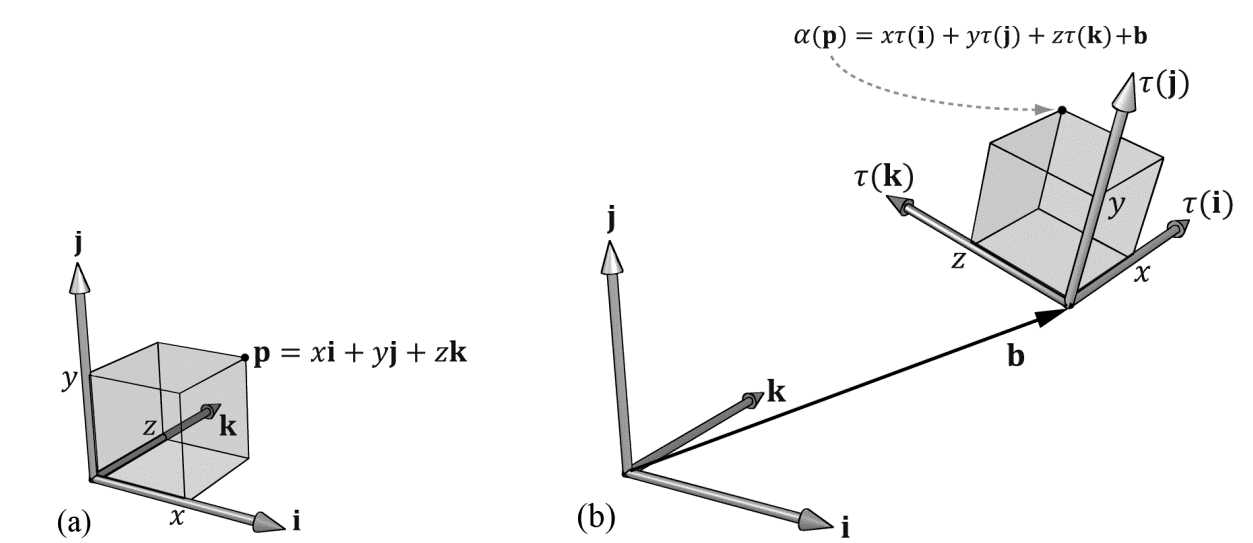
\includegraphics[width=\textwidth]{Images/4/3/4.Session.1.3.7}
            \caption {هندسه سطرهای یک ماتریس تبدیل آفین. نقطه تبدیل شده، $\alpha(\textbf{p})$)، به صورت ترکیبی خطی از بردارهای مبنا تبدیل شده \tau(\textbf{i})، \tau(\textbf{j}) و \tau(\textbf{k}) و آفست $\textbf{b}$ داده می شود.}
            \label{fig:4.Session.1.3.7}
        \end{figure}

        \begin{figure}[H]
            \centering
            \setlength{\belowcaptionskip}{-10pt}
            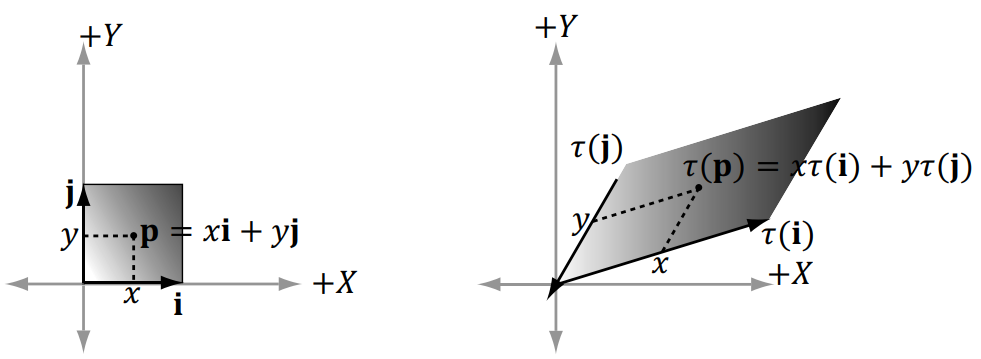
\includegraphics[width=0.8\textwidth]{Images/4/3/4.Session.1.3.8}
            \caption {برای تبدیل خطی که مربع را به متوازی الاضلاع می پیچد، نقطه تبدیل شده $\alpha(\textbf{p})=(x,y)$ به صورت ترکیبی خطی از بردارهای مبنا تبدیل شده \tau(\textbf{i}) و \tau(\textbf{j}) داده می شود.}
            \label{fig:4.Session.1.3.8}
        \end{figure}
    \end{spacing}
}


\section{\textbf{ترکیب تبدیلات}}
\label{sec:3.3}
{
    \Large
    \begin{spacing}{1.5}
        فرض کنید $\textbf{S}$ یک ماتریس مقیاس بندی، $\textbf{R}$ یک ماتریس دوران و $\textbf{T}$ یک ماتریس انتقال است.
        فرض کنید مکعبی داریم که از هشت رأس $\textbf{v}_{i}$ به ازای $i=0,1,...,7$ تشکیل شده است و
        می‌خواهیم این سه تبدیل را به صورت متوالی در هر راس اعمال کنیم. روش واضح برای انجام این کار گام به گام است:

        \begin{center}
            $((\textbf{v}_{i}\textbf{S})\textbf{R})\textbf{T}=(\textbf{v}\prime_{i}\textbf{R})\textbf{T}=\textbf{v}\prime\prime_{i}\textbf{T}=\textbf{v}\prime\prime\prime_{i}\hspace(5 mm)for i=0,1,\dots,7$
        \end{center}

        با این حال، از آنجایی که ضرب ماتریس شرکت پذیر است، در عوض می‌توانیم آن را به صورت معادل بنویسیم:

        \begin{center}
            $\textbf{v}_{i}(\textbf{SRT})=\textbf{v}\prime\prime\prime_{i}\hspace(5 mm)for i=0,1,\dots,7$
        \end{center}

        ما می توانیم ماتریس $\textbf{C}=\textbf{SRT}$ را به عنوان ماتریسی در نظر بگیریم که هر سه تبدیل را در یک ماتریس تبدیل خالص محصور می کند.
        به عبارت دیگر، ضرب ماتریس-ماتریس به ما اجازه می دهد تا تبدیل ها را به هم متصل کنیم.

        این پیامدهای عملکردی دارد. برای مشاهده این موضوع، فرض کنید یک شی سه بعدی از $20000$ نقطه تشکیل شده است و ما می خواهیم این سه تبدیل هندسی متوالی را روی جسم اعمال کنیم.
        با استفاده از روش گام به گام، به $20000\times 3$ ضرب ماتریس برداری نیاز داریم.
        از سوی دیگر، استفاده از رویکرد ماتریس ترکیبی به $20000$ ضرب بردار-ماتریس و $2$ ضرب ماتریس-ماتریس نیاز دارد. واضح است که دو ضرب اضافی ماتریس-ماتریس هزینه ارزانی برای صرفه جویی زیاد در ضرب ماتریس بردار است.

        \begin{point}{pnt:3.1}
            \Large
            مجدداً اشاره می کنیم که ضرب ماتریس جابجایی پذیر نیست. این حتی به صورت هندسی نیز دیده می شود.
            به عنوان مثال، یک دوران و سپس یک انتقال، که می‌توانیم آن را با حاصلضرب ماتریس $\textbf{RT}$ توصیف کنیم، به همان تبدیلی که همان انتقال به دنبال آن دوران یکسان است، یعنی $\textbf{TR}$، منجر نمی‌شود. شکل \ref{fig:4.Session.1.3.9} این را نشان می دهد.
        \end{point}

        \begin{figure}[H]
            \centering
            \setlength{\belowcaptionskip}{-10pt}
            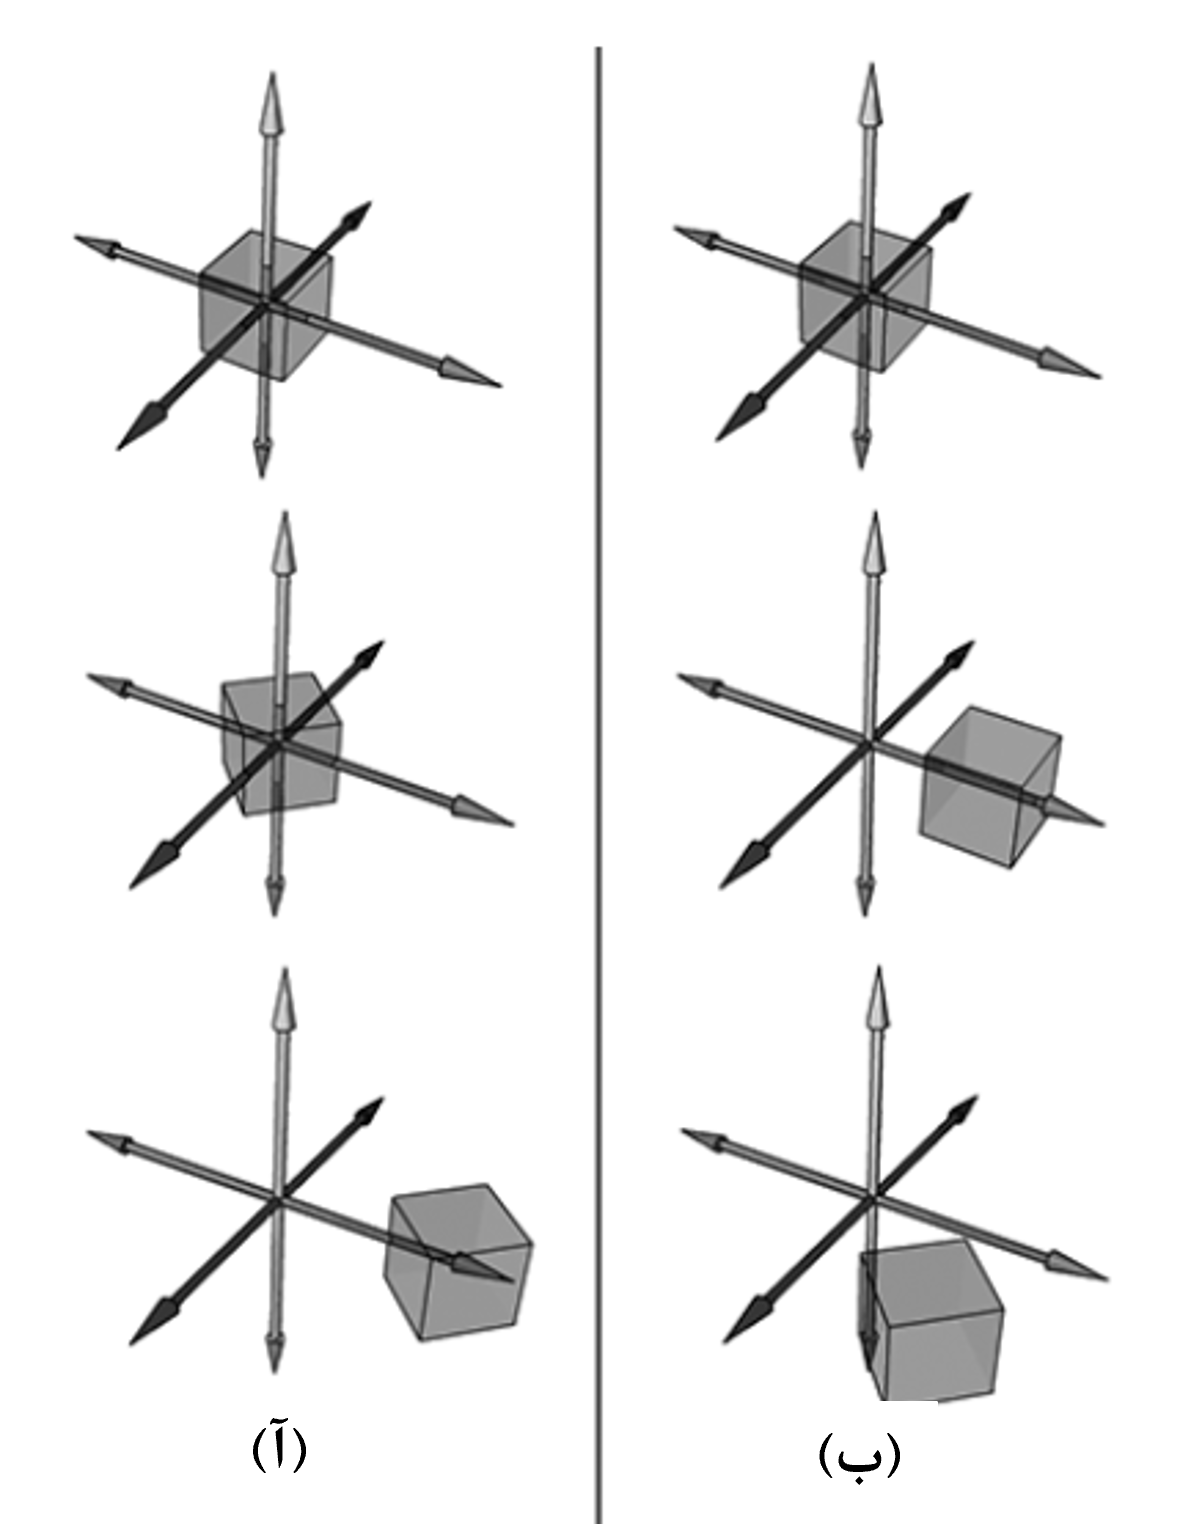
\includegraphics[width=0.8\textwidth]{Images/4/3/4.Session.1.3.9}
            \caption {(آ) ابتدا دوران و سپس انتقال. (ب) ابتدا انتقال و سپس دوران.}
            \label{fig:4.Session.1.3.9}
        \end{figure}
    \end{spacing}
}


\section{\textbf{تغییر تبدیلات مختصات}}
\label{sec:3.4}
{
    \Large
    \begin{spacing}{1.5}
        اسکالر $100$ درجه سانتیگراد نشان دهنده دمای آب در حال جوش نسبت به مقیاس سانتیگراد است.
        چگونه دمای یکسان آب جوش را نسبت به مقیاس فارنهایت توصیف کنیم؟ به عبارت دیگر، اسکالر نسبت به مقیاس فارنهایت که دمای آب در حال جوش را نشان می دهد چیست؟ برای انجام این تبدیل (یا تغییر فریم)، ​​باید بدانیم مقیاس های سانتیگراد و فارنهایت چگونه با هم ارتباط دارند.

        آنها به شرح روبرو مرتبط هستند:
        $T_{F}=\frac{\displaystyle 9}{\displaystyle 5}T_{C}+32^\circ$. بنابراین دمای آب در حال جوش نسبت به مقیاس فارنهایت با$T_{F}=\frac{\displaystyle 9}{\displaystyle 5}(100)^\circ+32^\circ=212^\circ F$ به دست می آید.

        این مثال نشان می‌دهد که ما می‌توانیم یک اسکالر $k$ که مقداری را نسبت به یک سیستم مختصات $A$ توصیف می‌کند،
        به یک اسکالر جدید $k\prime$ تبدیل کنیم که همان کمیت را نسبت به یک سیستم مختصات دیگر $B$ توصیف می‌کند،
        مشروط بر اینکه بدانیم سیستم مختصات $A$ و  $B$ چگونه به هم مرتبط هستند.
        در بخش‌های فرعی بعدی، ما به یک مشکل مشابه نگاه می‌کنیم، اما به جای اسکالرها، به چگونگی تبدیل مختصات یک نقطه/بردار نسبت به یک سیستم مختصات به مختصات نسبت به یک سیستم مختصات متفاوت علاقه‌مندیم (شکل \ref{fig:4.Session.1.3.10} را ببینید).
        تبدیل مختصات را از یک سیستم مختصات به مختصات سیستم مختصات دیگر را تبدیل مختصات می نامیم.
        شایان ذکر است که در تغییر تبدیل مختصات، هندسه را تغییر نمیدهیم. در عوض، ما چارچوب مرجع را تغییر می دهیم، که بنابراین نمایش مختصات هندسه را تغییر می دهد.
        این برخلاف طرز فکر ما در مورد دوران ها، انتقال ها و مقیاس بندی است، که در آن به حرکت فیزیکی یا تغییر شکل هندسه فکر می کنیم.
        در گرافیک کامپیوتری سه بعدی، ما از چند سیستم مختصات استفاده می کنیم، بنابراین باید بدانیم که چگونه از یک سیستم تبدیل کنیم.
        به دیگری. از آنجایی که مکان ویژگی نقاط است، اما نه بردارها، تغییر تبدیل مختصات برای نقاط و بردارها متفاوت است.

        \begin{figure}[H]
            \centering
            \setlength{\belowcaptionskip}{-10pt}
            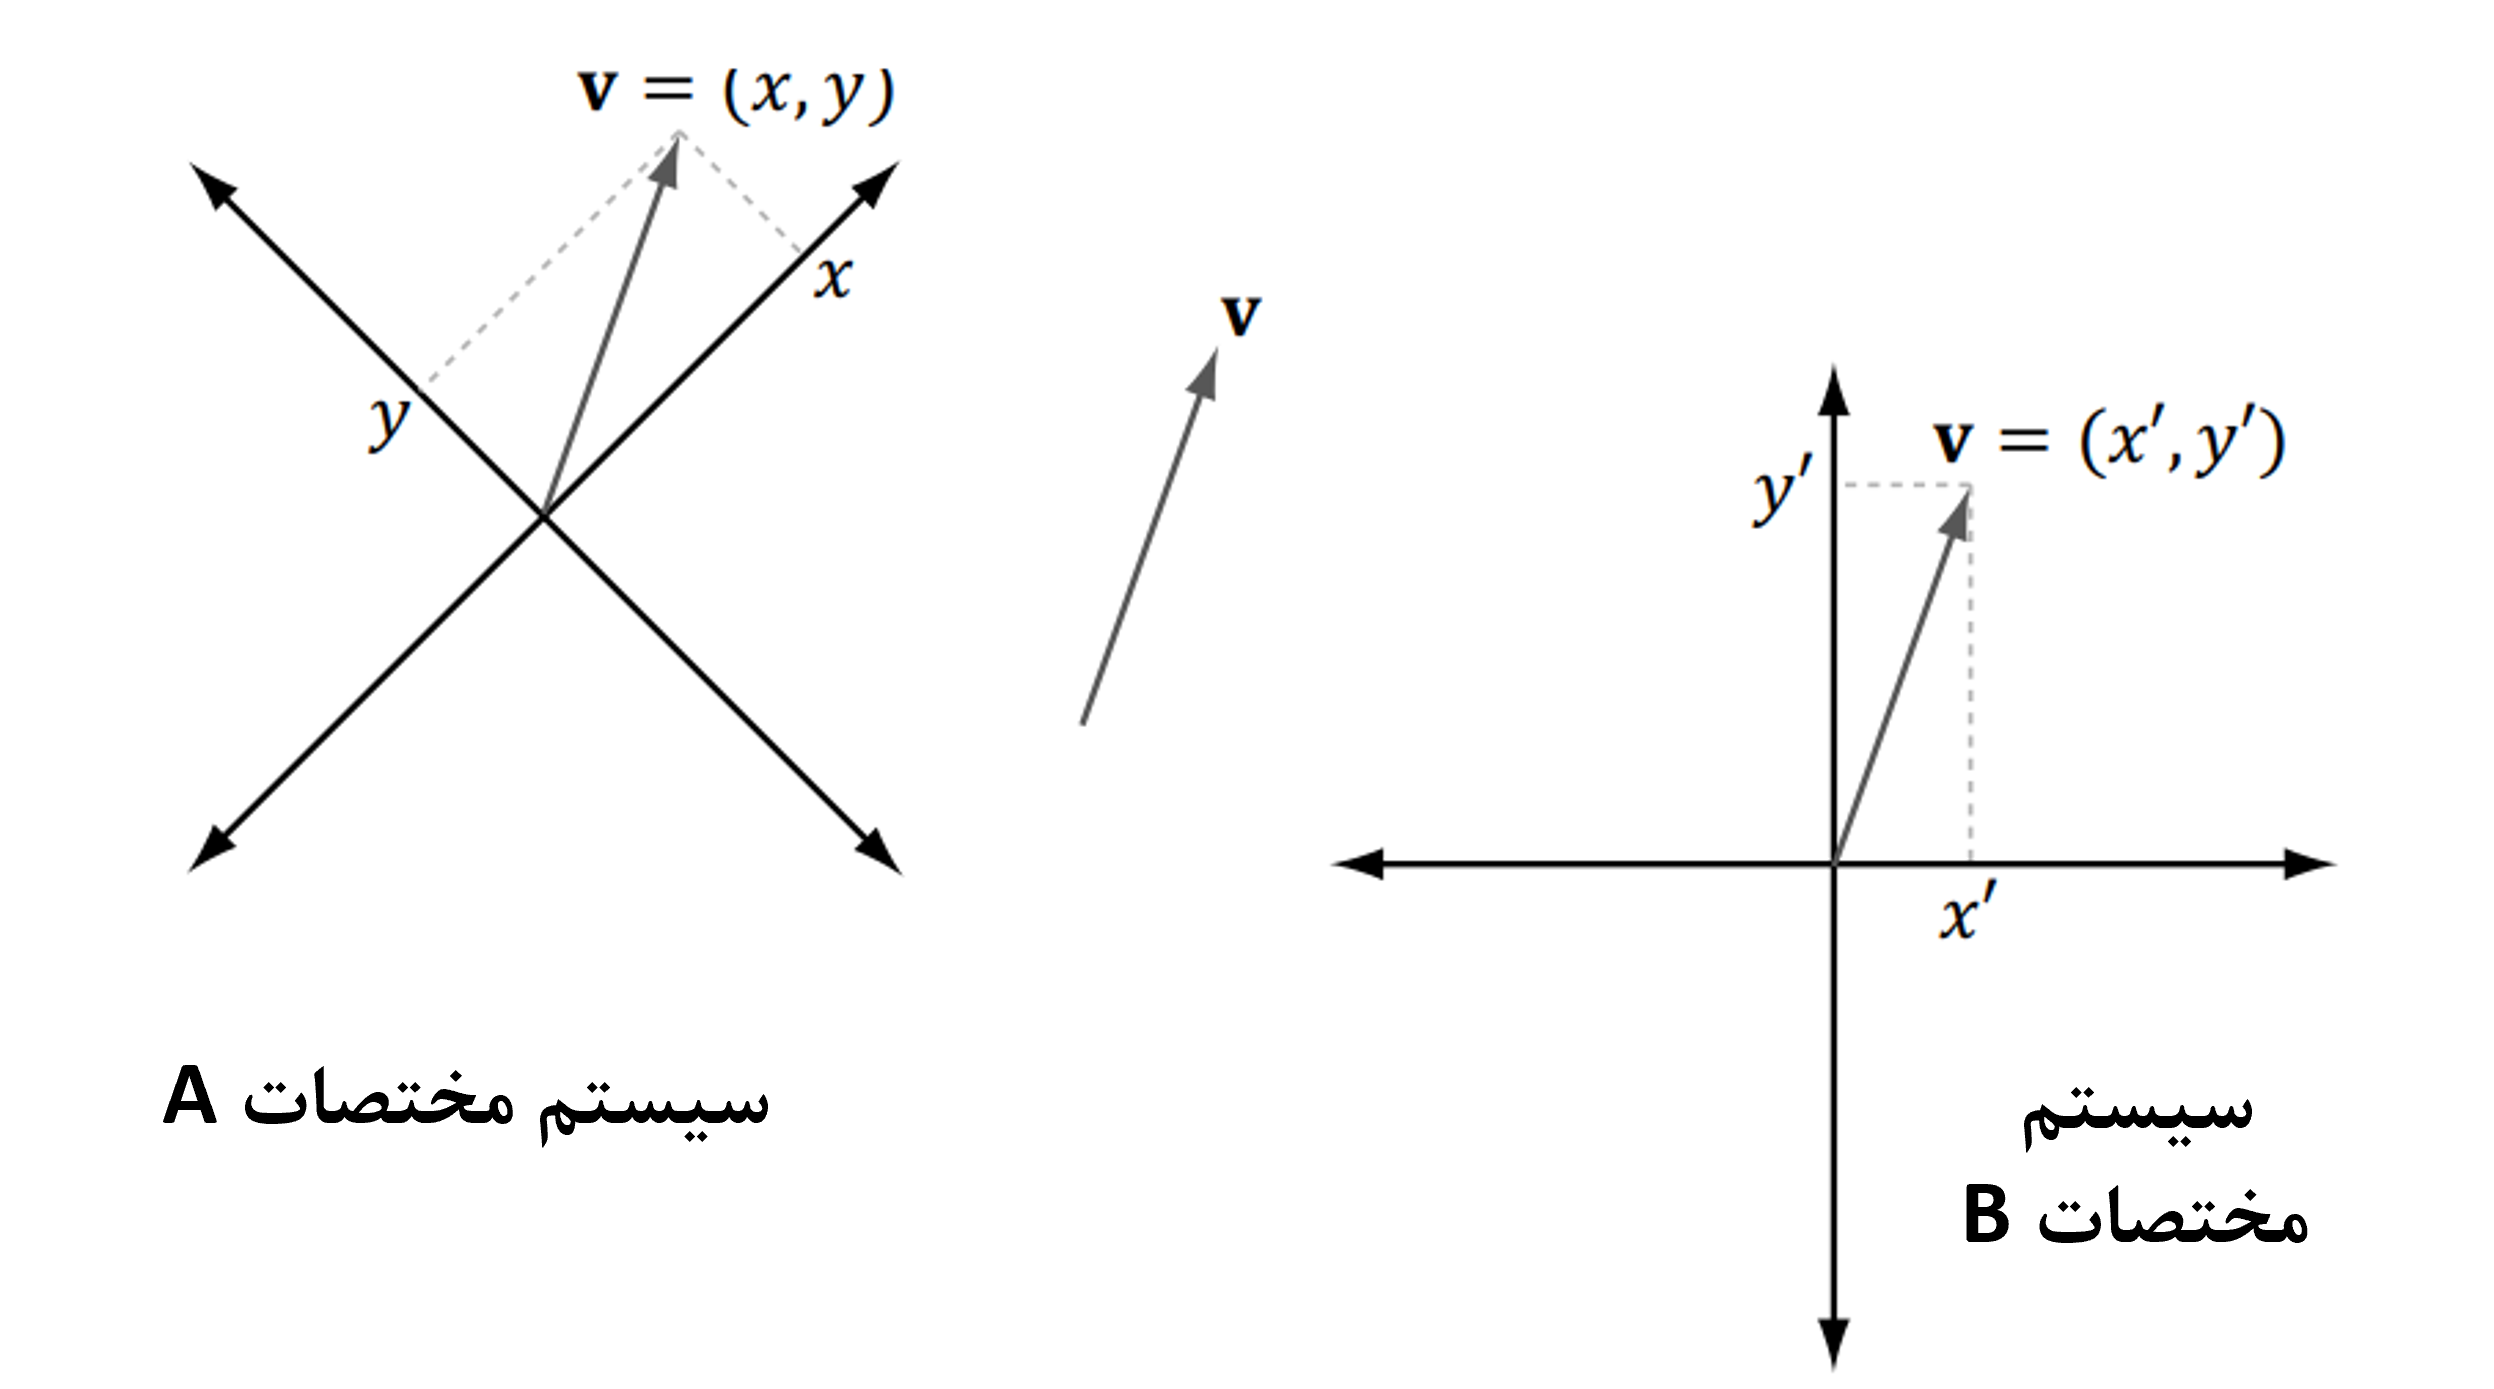
\includegraphics[width=0.8\textwidth]{Images/4/3/4.Session.1.3.10}
            \caption {همان بردار $\textbf{v}$ زمانی که نسبت به سیستم متخصات های مختلف توضیح داده می شود مختصات متفاوتی دارد. مختصات $(x, y)$ نسبت به سیستم متخصات $A$ و مختصات $(x\prime, y\prime)$ نسبت به سیستم متخصات $B$ دارد.}
            \label{fig:4.Session.1.3.10}
        \end{figure}
    \end{spacing}
}

\subsection{\textbf{بردار ها}}
{
    \Large
    \begin{spacing}{1.5}
        شکل \ref{fig:4.Session.1.3.11} را در نظر بگیرید که در آن دو سیستم مختصات $A$ و $B$ و یک بردار $\textbf{p}$ داریم.
        فرض کنید مختصات $\textbf{p}$، $\textbf{p}_{B}=(x, y)$ نسبت به سیستم مختصات $A$ به ما داده شده است
        و می خواهیم مختصات $\textbf{p}$، $\textbf{p}_{B}=(x\prime, y\prime)$ را نسبت به سیستم مختصات $B$ پیدا کنیم.
        به عبارت دیگر، با توجه به مختصات با شناسایی یک بردار نسبت به یک سیستم مختصات، چگونه مختصاتی را پیدا کنیم که همان بردار را نسبت به یک سیستم مختصات دیگر مشخص می کند؟

        \begin{figure}[H]
            \centering
            \setlength{\belowcaptionskip}{-10pt}
            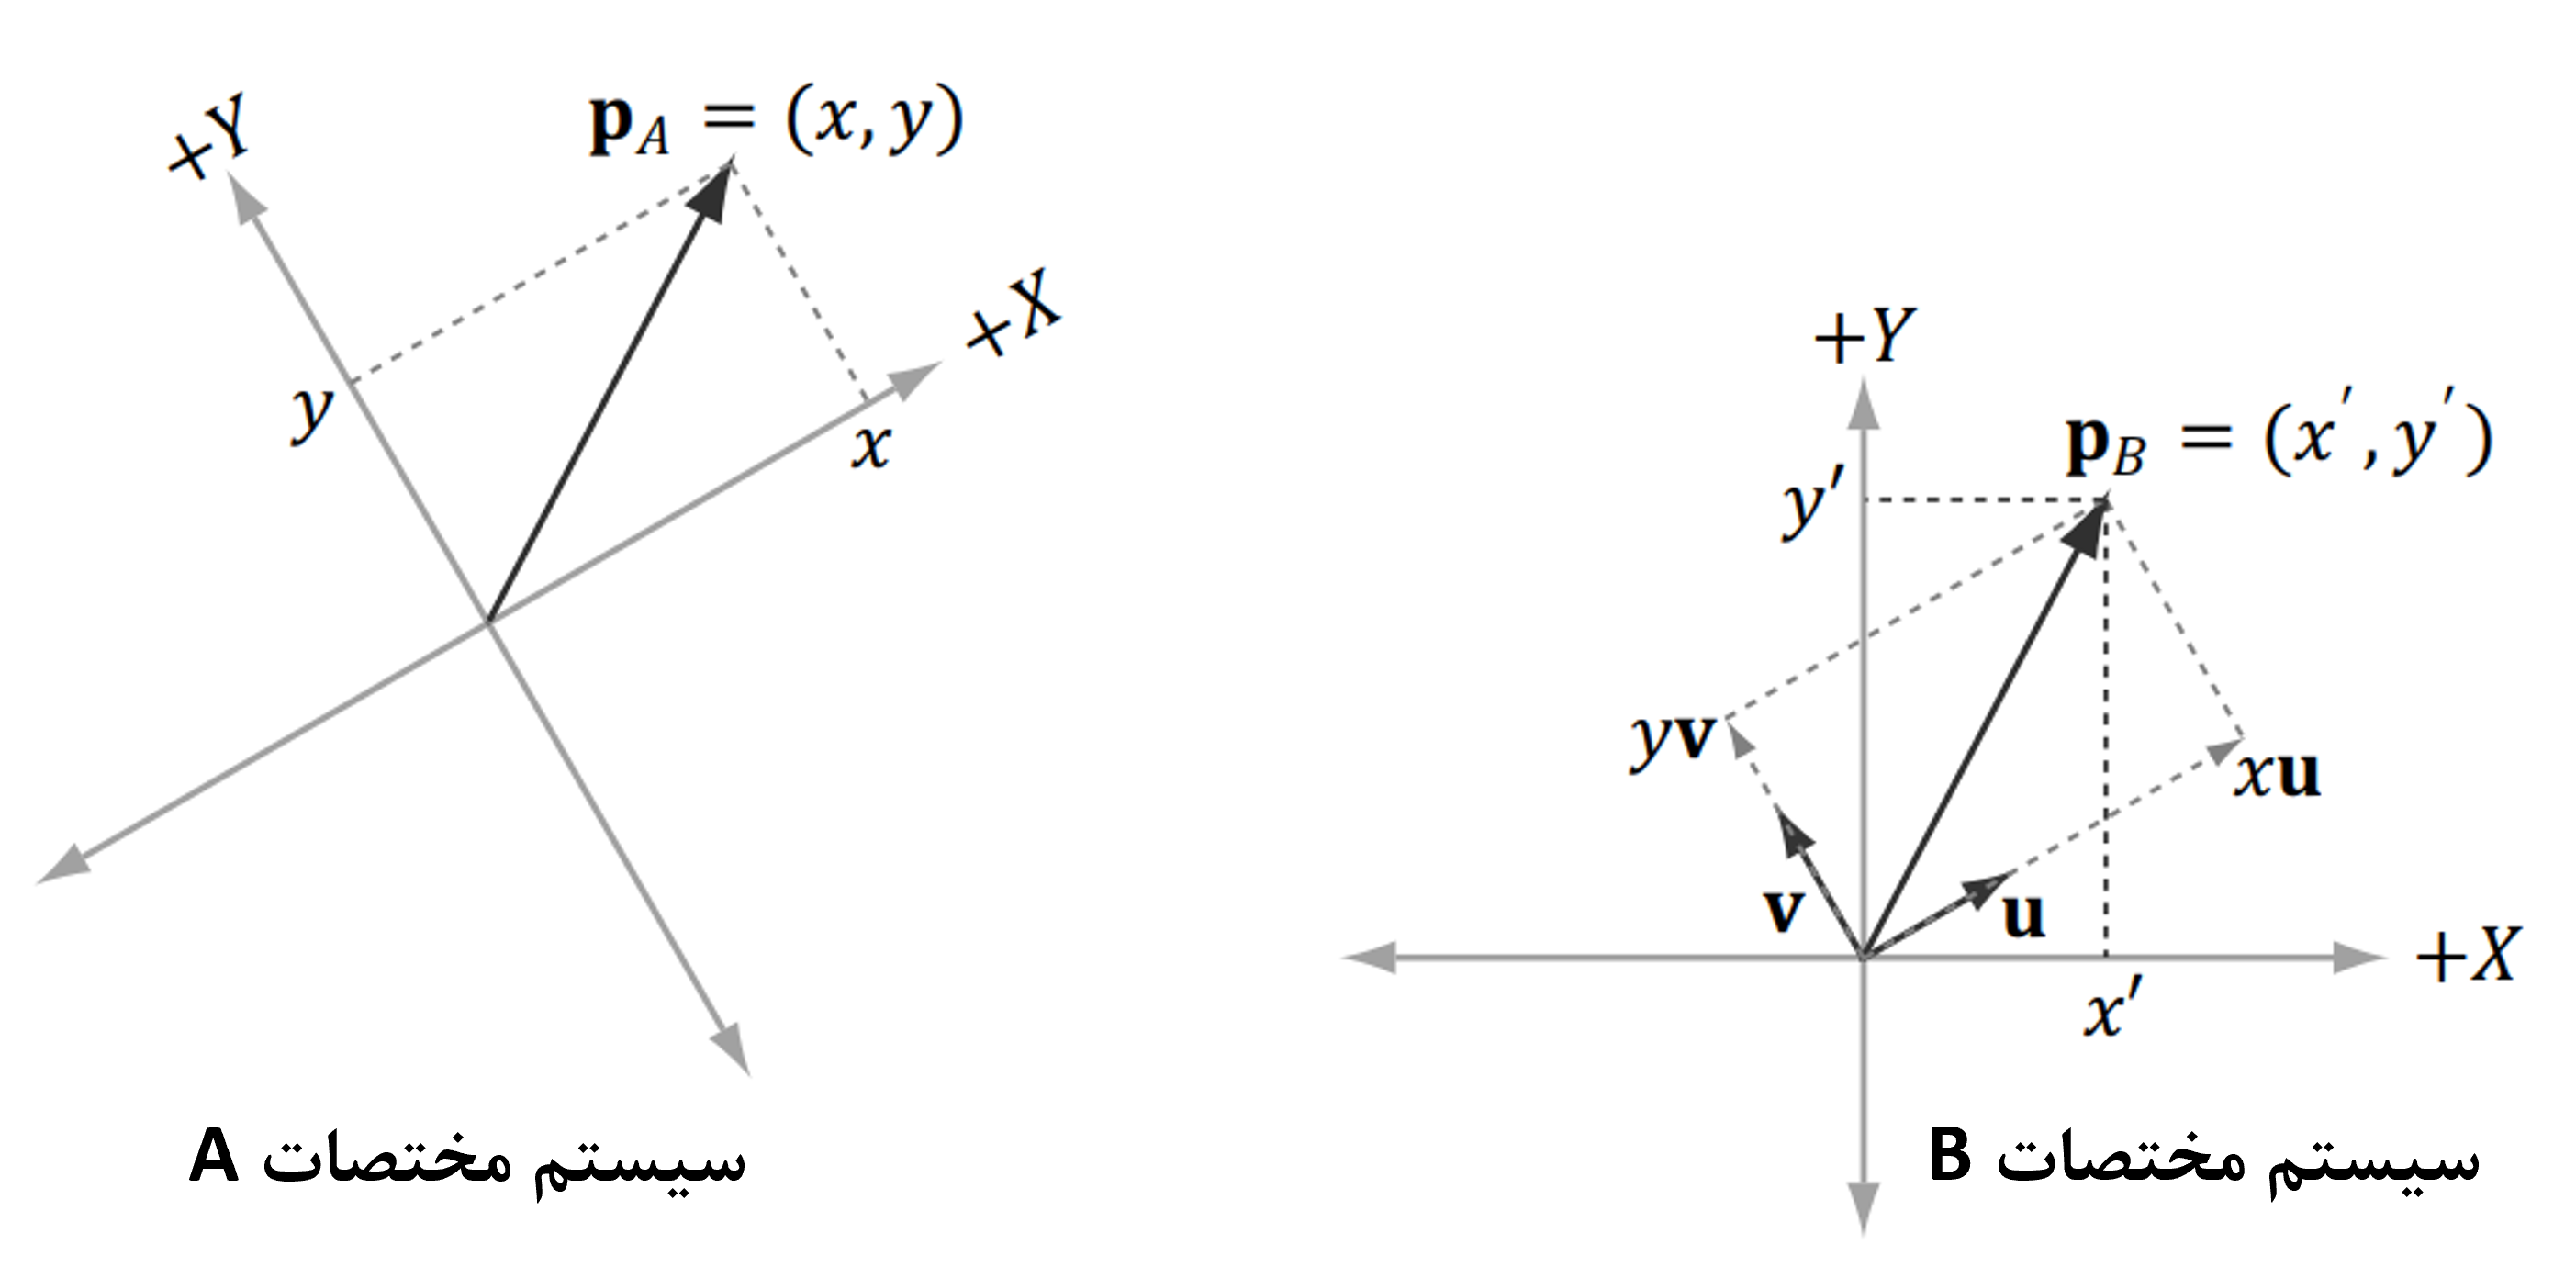
\includegraphics[width=0.8\textwidth]{Images/4/3/4.Session.1.3.11}
            \caption {هندسه یافتن مختصات $\textbf{p}$ نسبت به سیستم مختصات $B$.}
            \label{fig:4.Session.1.3.11}
        \end{figure}

        از شکل \ref{fig:4.Session.1.3.11}، مشخص است که

        \begin{center}
            $\textbf{p}=x\textbf{u}+y\textbf{v}$
        \end{center}

        که در آن $\textbf{u}$ و $\textbf{v}$ بردارهای واحدی هستند که به ترتیب در امتداد محورهای $x$ و $y$ سیستم مختصات $A$ هدف قرار می گیرند.
        با بیان هر بردار در معادله بالا در مختصات سیستم مختصات $B$ به دست می آوریم:

        \begin{center}
            $\textbf{p}_{B}=x\textbf{u}_{B}+y\textbf{v}_{B}$
        \end{center}

        بنابراین، اگر $\textbf{p}_{A}=(x, y)$ به ما داده شود و مختصات بردارهای $\textbf{u}$ و $\textbf{v}$ را نسبت به سیستم مختصات $B$ بدانیم،
        یعنی اگر $\textbf{u}_{B}=(u_{x}, u_{y})$ و $\textbf{v}_{B}=(v_{x}, v_{y})$ را بدانیم، سپس ما همیشه می توانیم $\textbf{p}_{B}=(x\prime, y\prime)$ را پیدا کنیم.

        تعمیم به سه بعدی، اگر $\textbf{p}_{A}=(x, y, z)$، پس

        \begin{center}
            $\textbf{p}_{B}=x\textbf{u}_{B}+y\textbf{v}_{B}+z\textbf{w}_{B}$
        \end{center}

        که در آن $\textbf{u}$، $\textbf{v}$ و $\textbf{w}$ بردارهای واحدی هستند که به ترتیب در امتداد محورهای $x$، $y$ و $z$ سیستم متخصات $A$ هدف قرار می‌گیرند.
    \end{spacing}
}

\subsection{\textbf{نقاط}}
{
    \Large
    \begin{spacing}{1.5}
        تغییر تبدیل مختصات برای نقاط کمی متفاوت از آن برای بردار است.
        این به این دلیل است که مکان برای نقاط مهم است، بنابراین ما نمی‌توانیم نقاط را همانطور که بردارهای شکل 3.11 را نتقال دادیم، انتقال دهیم.

        \begin{figure}[H]
            \centering
            \setlength{\belowcaptionskip}{-10pt}
            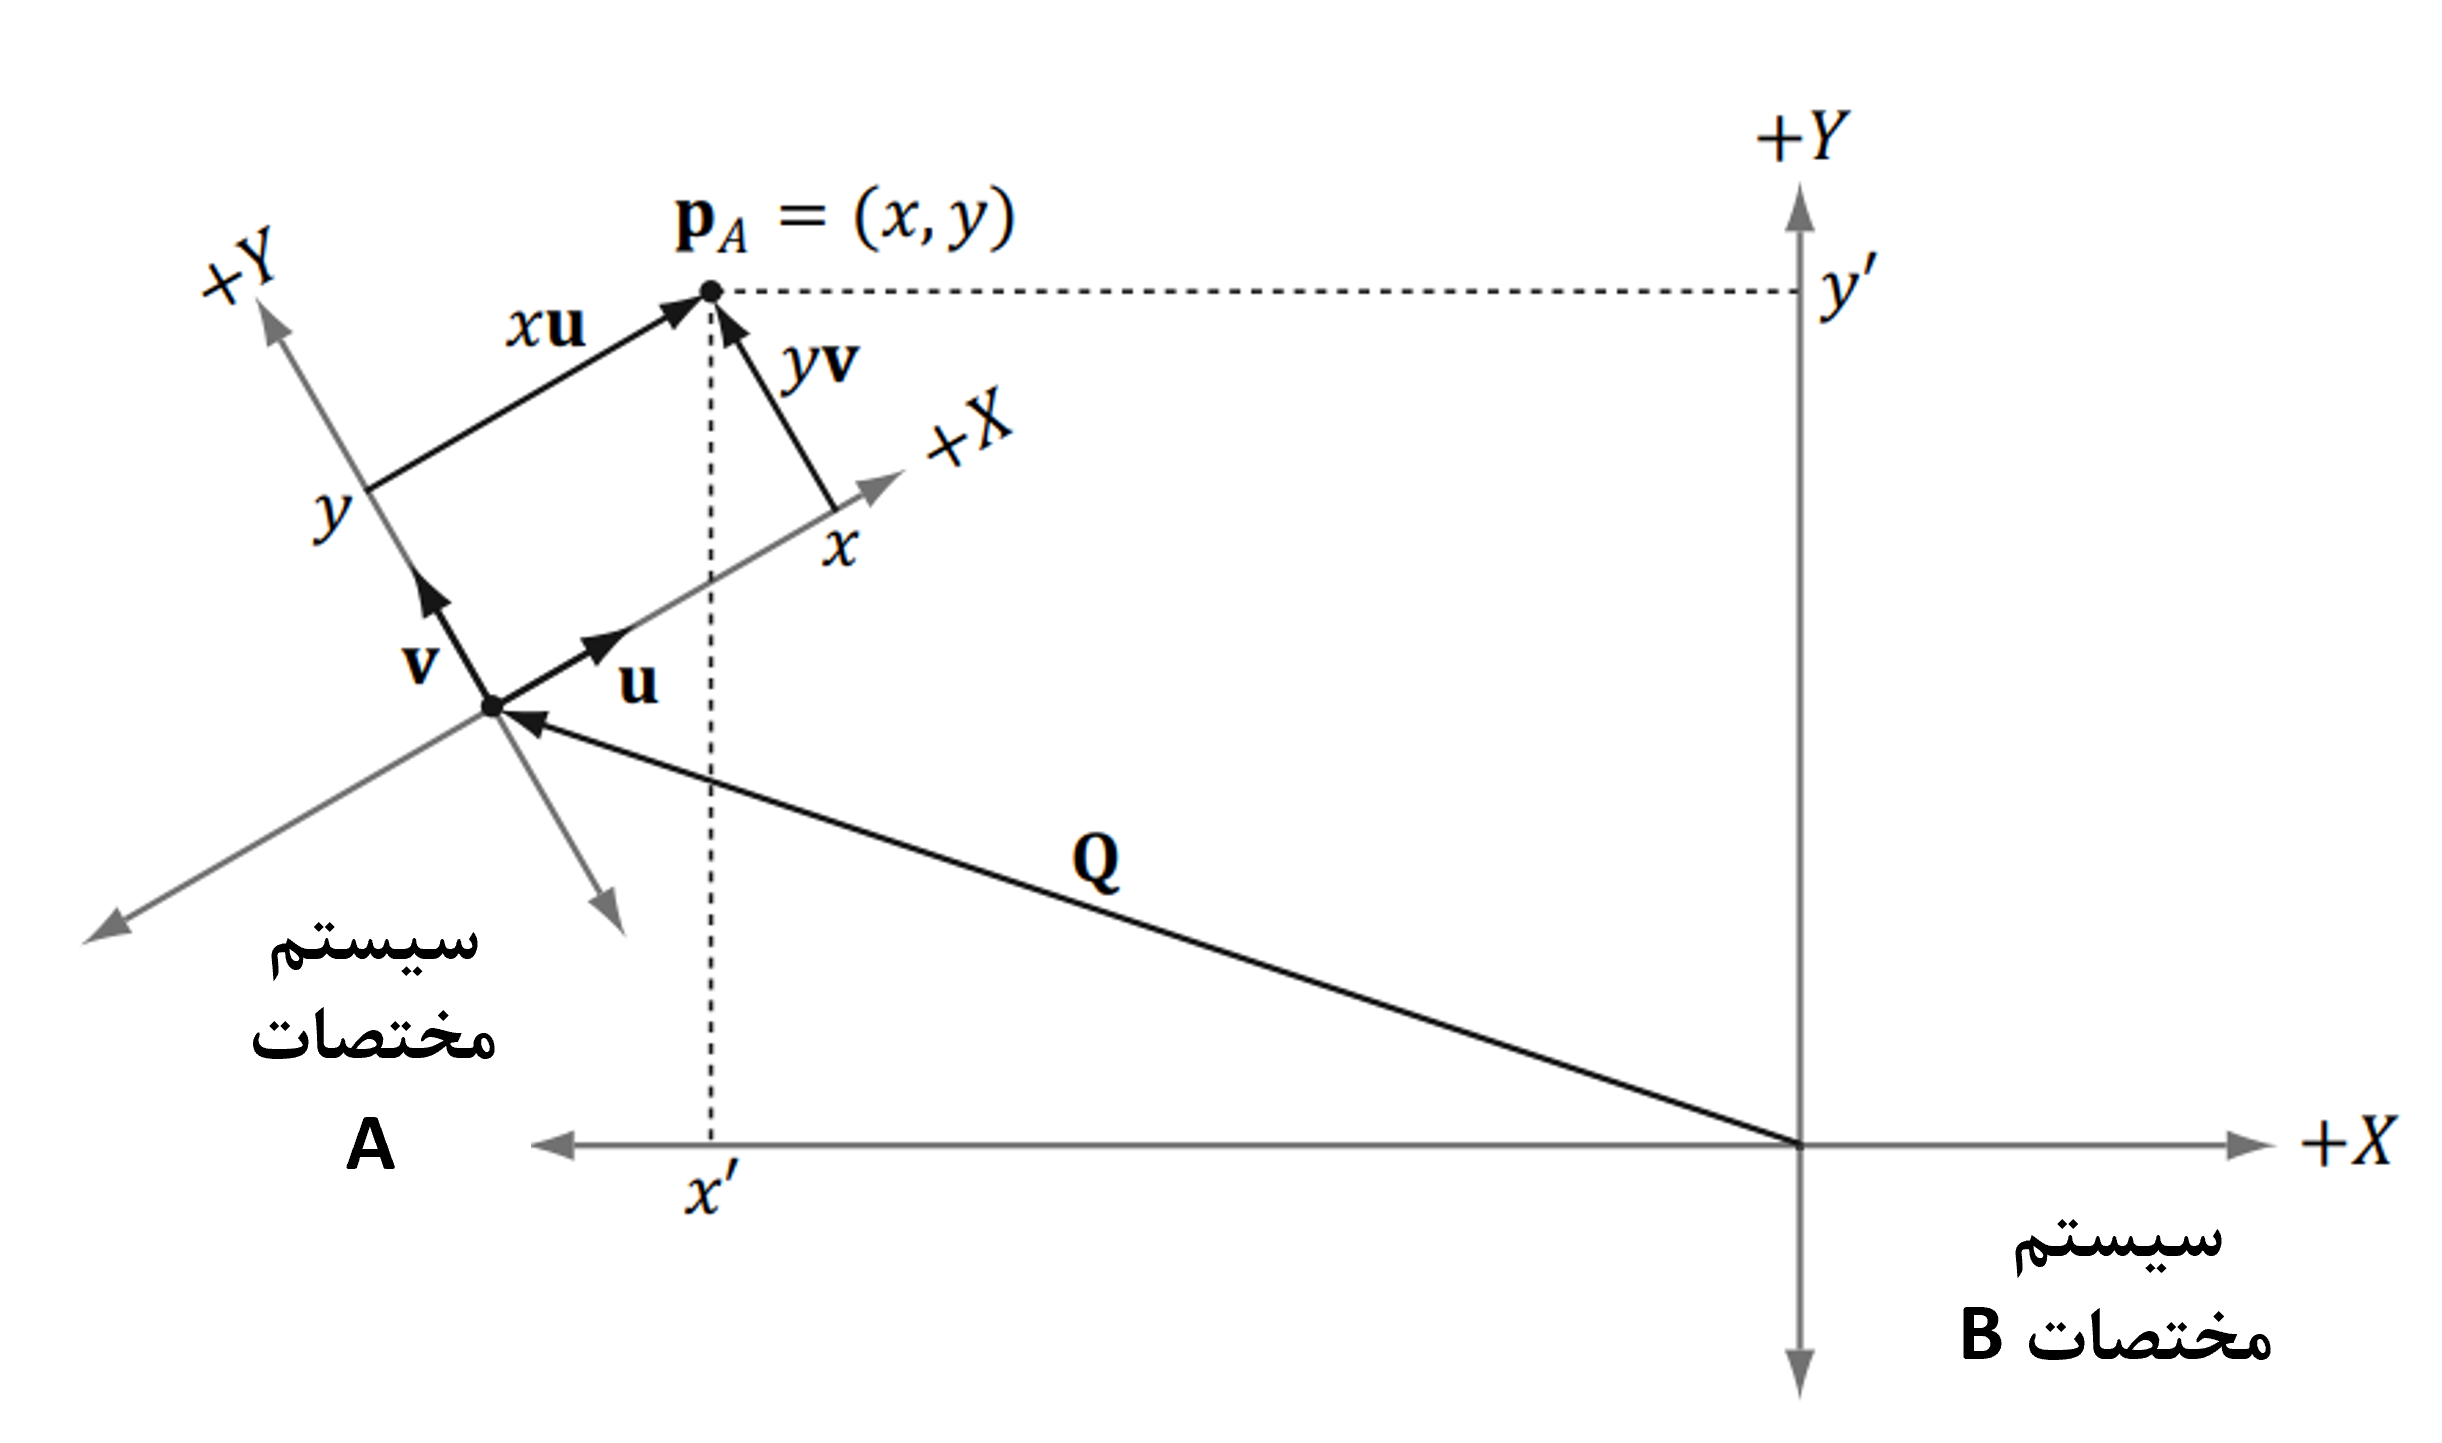
\includegraphics[width=0.8\textwidth]{Images/4/3/4.Session.1.3.12}
            \caption {هندسه یافتن مختصات $\textbf{p}$ نسبت به سیستم مختصات $B$.}
            \label{fig:4.Session.1.3.12}
        \end{figure}

        شکل \ref{fig:4.Session.1.3.12} وضعیت را نشان می دهد و می بینیم که نقطه $\textbf{p}$ را می توان با معادله بیان کرد:

        \begin{center}
            $\textbf{p}=x\textbf{u}+y\textbf{v}+\textbf{Q}$
        \end{center}

        که در آن $\textbf{u}$ و $\textbf{v}$ بردارهای واحدی هستند که به ترتیب در امتداد محورهای $x$ و $y$ سیستم متخصات $A$ هدف قرار می گیرند و $\textbf{Q}$ مبدا سیستم مختصات $A$ است.
        با بیان هر بردار/نقطه در معادله بالا در مختصات سیستم مختصات $B$ به دست می آوریم:

        \begin{center}
            $\textbf{p}_{B}=x\textbf{u}_{B}+y\textbf{v}_{B}+\textbf{Q}_{B}$
        \end{center}

        بنابراین، اگر $\textbf{p}_{A}=(x, y)$ به ما داده شود و مختصات بردارهای $\textbf{u}$ و $\textbf{v}$ و مبدأ $\textbf{Q}$ را نسبت به سیستم مختصات $B$ بدانیم، یعنی اگر $\textbf{u}_{B}=(u_{x}, u_{y})$ ، $\textbf{v}_{B}=(v_{x}, v_{y})$ و $\textbf{Q}_{B}=(Q_{x}, Q_{y})$ را بدانیم، سپس ما همیشه می توانیم $\textbf{p}_{B}=(x\prime, y\prime)$ را پیدا کنیم.

        تعمیم به سه بعدی، اگر $\textbf{p}_{A}=(x, y, z)$، پس

        \begin{center}
            $\textbf{p}_{B}=x\textbf{u}_{B}+y\textbf{v}_{B}+z\textbf{w}_{B}+\textbf{Q}_{B}$
        \end{center}

        که در آن $\textbf{u}$، $\textbf{v}$ و $\textbf{w}$ بردارهای واحدی هستند که به ترتیب در امتداد محورهای $x$، $y$ و $z$ سیستم متخصات $A$ هدف قرار می گیرند و $\textbf{Q}$ مبدا سیستم متخصات $A$ است.
    \end{spacing}
}

\subsection{\textbf{نمایش ماتریسی}}
{
    \Large
    \begin{spacing}{1.5}
        برای بازبینی، بردار و تغییر نقطه تبدیل مختصات عبارتند از:

        \begin{flushleft}
            $(x\prime,y\prime,z\prime)=x\textbf{u}_{B}+y\textbf{v}_{B}+z\textbf{w}_{B}$ \rl{برای بردار ها}\\
            $\textbf{p}_{B}=x\textbf{u}_{B}+y\textbf{v}_{B}+z\textbf{w}_{B}+\textbf{Q}_{B}$ \rl{برای نقطه ها}
        \end{flushleft}

        اگر از مختصات همگن استفاده کنیم، می‌توانیم بردارها و نقاط را با یک معادله کنترل کنیم:

        \begin{eqtn}{eqtn:3.8}
            \centering
            $(x\prime,y\prime,z\prime,w)=x\textbf{u}_{B}+y\textbf{v}_{B}+z\textbf{w}_{B}+w\textbf{Q}_{B}$
        \end{eqtn}

        اگر $w=0$ باشد، این معادله به تغییر تبدیل مختصات برای بردارها کاهش می یابد.
        اگر $w=1$ باشد، این معادله به تغییر تبدیل مختصات برای نقاط کاهش می یابد.
        مزیت معادله \ref{eqtn:3.8} این است که هم برای بردارها و هم برای نقاط کار می کند، مشروط بر اینکه مختصات $w$ را به درستی تنظیم کنیم.
        ما دیگر نیازی به دو معادله نداریم (یکی برای بردارها و دیگری برای نقاط). معادله \ref{eqtn:2.3} می گوید که می توانیم معادله \ref{eqtn:3.8} را به زبان ماتریس ها بنویسیم:

        \begin{eqtn}{eqtn:3.9}
            \begin{equation*}
                \centering
                \begin{split}
                [x\prime,y\prime,z\prime,w]
                    &=[x,y,z,w]\begin{bmatrix}
                                   \leftarrow & \textbf{u}_{B} & \rightarrow \\
                                   \leftarrow & \textbf{v}_{B} & \rightarrow \\
                                   \leftarrow & \textbf{w}_{B} & \rightarrow \\
                                   \leftarrow & \textbf{Q}_{B} & \rightarrow
                    \end{bmatrix} \\
                    &=[x,y,z,w]\begin{bmatrix}
                                   u_{x} & u_{y} & u_{z} & 0 \\
                                   v_{x} & v_{y} & v_{z} & 0 \\
                                   w_{x} & w_{y} & w_{z} & 0 \\
                                   Q_{x} & Q_{y} & Q_{z} & 1
                    \end{bmatrix} \\
                    &=x\textbf{u}_{B}+y\textbf{v}_{B}+z\textbf{w}_{B}+w\textbf{Q}_{B}
                \end{split}
            \end{equation*}
            \centering
        \end{eqtn}

        جایی که $\textbf{Q}_{B}=(Q_{x}, Q_{y}, Q_{z}, 1)$، $\textbf{u}_{B}=(u_{x}, u_{y}, u_{z}, 0)$، $\textbf{v}_{B}=(v_{x}, v_{y}, v_{z}, 0)$، و $\textbf{Q}_{B}=(w_{x}, w_{y}, w_{z}, 0)$ مبدا و محورهای سیستم مختصات A با مختصات همگن نسبت به سیستم مختصات B را توصیف می‌کند.
        ماتریس $4\times 4$ را در معادله \ref{eqtn:3.9} تغییر ماتریس مختصات یا تغییر ماتریس سیستم مختصات می نامیم و می گوییم مختصات سیستم مختصات $A$ را به مختصات سیستم مختصات $B$ تبدیل می کند (یا نقشه میکند).
    \end{spacing}
}

\subsection{\textbf{شرکت پذیری و تغییر ماتریس مختصات}}
{
    \Large
    \begin{spacing}{1.5}
        حال فرض کنید سه فریم $F$، $G$ و $H$ داریم. علاوه بر این، اجازه دهید $\textbf{A}$
        تغییر ماتریس سیستم مختصات از $F$ به $G$ باشد،
        و اجازه دهید $\textbf{B}$ تغییر ماتریس فریم از $G$ به $H$ باشد. فرض کنید مختصات $\textbf{p}_{F}$ را داریم.
        بردار نسبت به سیستم مختصات $F$ و مختصات همان بردار را نسبت به فریم $H$ می خواهیم، ​​یعنی $\textbf{p}_{H}$ را می خواهیم.
        یکی از راه های انجام این کار مرحله به مرحله است:

        \begin{center}
            $(\textbf{p}_{F}\textbf{A})\textbf{B}=\textbf{p}_{H}$ \\
            $(\textbf{p}_{G})\textbf{B}=\textbf{p}_{H}$
        \end{center}

        با این حال، از آنجایی که ضرب ماتریس شرکت پذیر است، می توانیم $(\textbf{p}_{F}\textbf{A})\textbf{B}=\textbf{p}_{H}$ را به صورت زیر بازنویسی کنیم:

        \begin{center}
            $\textbf{p}_{F}(\textbf{A}\textbf{B})=\textbf{p}_{H}$
        \end{center}

        از این نظر، حاصلضرب ماتریس $\textbf{C}=\textbf{AB}$ را می توان به عنوان تغییر ماتریس سیستم مختصات از F مستقیم به H در نظر گرفت.
        این تأثیرات A و B را در یک ماتریس خالص ترکیب می کند. (این ایده مانند ترکیب توابع است.)

        این پیامدهای عملکردی دارد. برای مشاهده این موضوع، فرض کنید که یک شی سه بعدی از $20000$ نقطه تشکیل شده است و ما می خواهیم دو تغییر متوالی تغییر قاب را روی شی اعمال کنیم.
        با استفاده از رویکرد گام به گام، به $20000\times 2$ ضرب ماتریس برداری نیاز داریم. از سوی دیگر، استفاده از رویکرد ماتریس ترکیبی به $20000$ ضرب بردار-ماتریس و $1$ ضرب ماتریس-ماتریس برای ترکیب دو تغییر ماتریس سیستم مختصات نیاز دارد.
        واضح است که یک ضرب ماتریس-ماتریس اضافی قیمت ارزانی برای صرفه جویی زیاد در ضرب ماتریس بردار است.

        \begin{point}{pnt:3.1}
            \Large
            باز هم، ضرب ماتریس جابجایی پذیر نیست، بنابراین انتظار داریم که AB و BA تبدیل ترکیبی یکسانی را نشان ندهند.
            به طور دقیق تر، ترتیبی که در آن ماتریس ها را ضرب می کنید، ترتیبی است که در آن تبدیل ها اعمال می شود و به طور کلی، این یک فرآیند جابجایی پذیر نیست.
        \end{point}

    \end{spacing}
}

\subsection{\textbf{معکوس ها و تغییر ماتریس های مختصات}}
{
    \Large
    \begin{spacing}{1.5}
        فرض کنید که $\textbf{p}_{B}$ (مختصات یک بردار $\textbf{p}$ نسبت به سیستم مختصات $B$) به ما داده می شود، و ماتریس مختصات $\textbf{M}$ از سیستم مختصات $A$ به سیستم مختصات $B$ به ما داده می شود.
        یعنی$\textbf{p}_{B}=\textbf{p}_{A}\textbf{M}$. ما می خواهیم برای $\textbf{p}_{A}$ حل کنیم.
        به عبارت دیگر، به جای نگاشت از سیستم مختصات $A$ به سیستم مختصات $B$، ماتریس مختصاتی را می خواهیم که ما را از $B$ به $A$ نگاشت می کند.
        برای یافتن این ماتریس، فرض کنید $\textbf{M}$ معکوس پذیر است (یعنی $\textbf{M}^{-1}$ وجود دارد). ما میتوانیم برای \textbf{p}_{A} مانند این حل کنیم:

        \begin{flushleft}
            \lr{$\textbf{p}_{B}=\textbf{p}_{A}\textbf{M}$\\
                $\textbf{p}_{B}\textbf{M}^{-1}=\textbf{p}_{A}\textbf{M}\textbf{M}^{-1}$\hspace{19 mm} \rl{(ضرب دو طرف معادله در $\textbf{M}^{-1}$)}\\
                $\textbf{p}_{B}\textbf{M}^{-1}=\textbf{p}_{A}\textbf{I}$\hspace{33 mm} \rl{($\textbf{M}\textbf{M}^{-1}=\textbf{I}$، با تعریف معکوس.)}\\
                $\textbf{p}_{B}\textbf{M}^{-1}=\textbf{p}_{A}$\hspace{35 mm} \rl{($\textbf{p}_{A}\textbf{I}=\textbf{p}_{A}$، با تعریف ماتریس همانی.)}
            }
        \end{flushleft}

        بنابراین ماتریس $\textbf{M}^{-1}$ تغییر ماتریس مختصات از $B$ به $A$ است.

        شکل \ref{fig:4.Session.1.3.13} رابطه بین تغییر ماتریس مختصات و معکوس آن را نشان می دهد.
        همچنین توجه داشته باشید که تمام تغییرات نگاشت سیستم مختصات که در این کتاب انجام می‌دهیم، معکوس خواهند بود، بنابراین دیگر نگران وجود معکوس نخواهیم بود.

        \begin{figure}[H]
            \centering
            \setlength{\belowcaptionskip}{-10pt}
            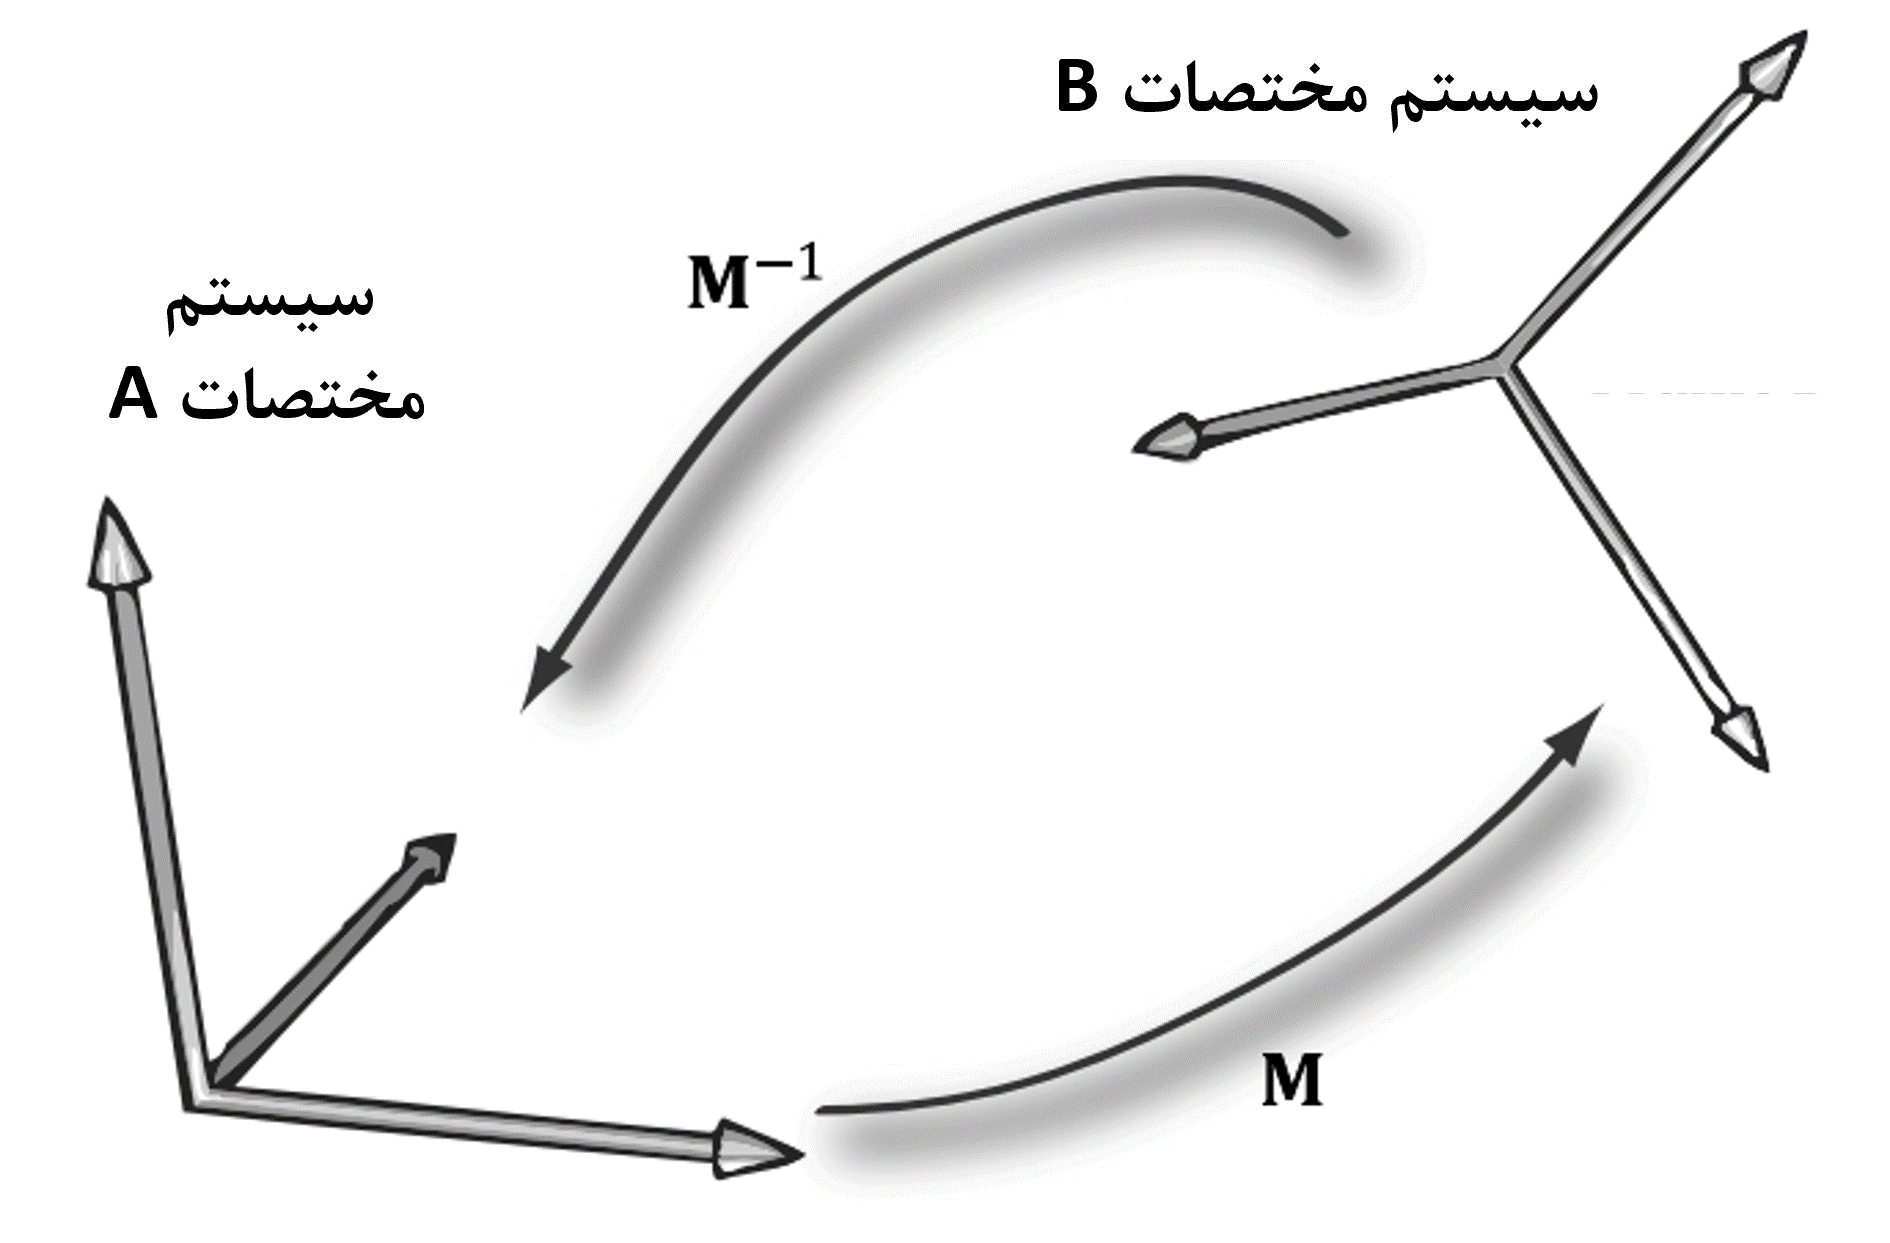
\includegraphics[width=0.5\textwidth]{Images/4/3/4.Session.1.3.13}
            \caption {$\textbf{M}$، $A$ را به $B$ و $\textbf{M}^{-1}$ از $B$ به $A$ نگاشت می کند.}
            \label{fig:4.Session.1.3.13}
        \end{figure}

        شکل \ref{fig:4.Session.1.3.14} نشان می دهد که چگونه ویژگی معکوس ماتریس $\textbf{AB}^{-1}=\textbf{B}^{-1}\textbf{A}^{-1}$ را می توان بر حسب تغییر ماتریس های مختصات تفسیر کرد.

        \begin{figure}[H]
            \centering
            \setlength{\belowcaptionskip}{-10pt}
            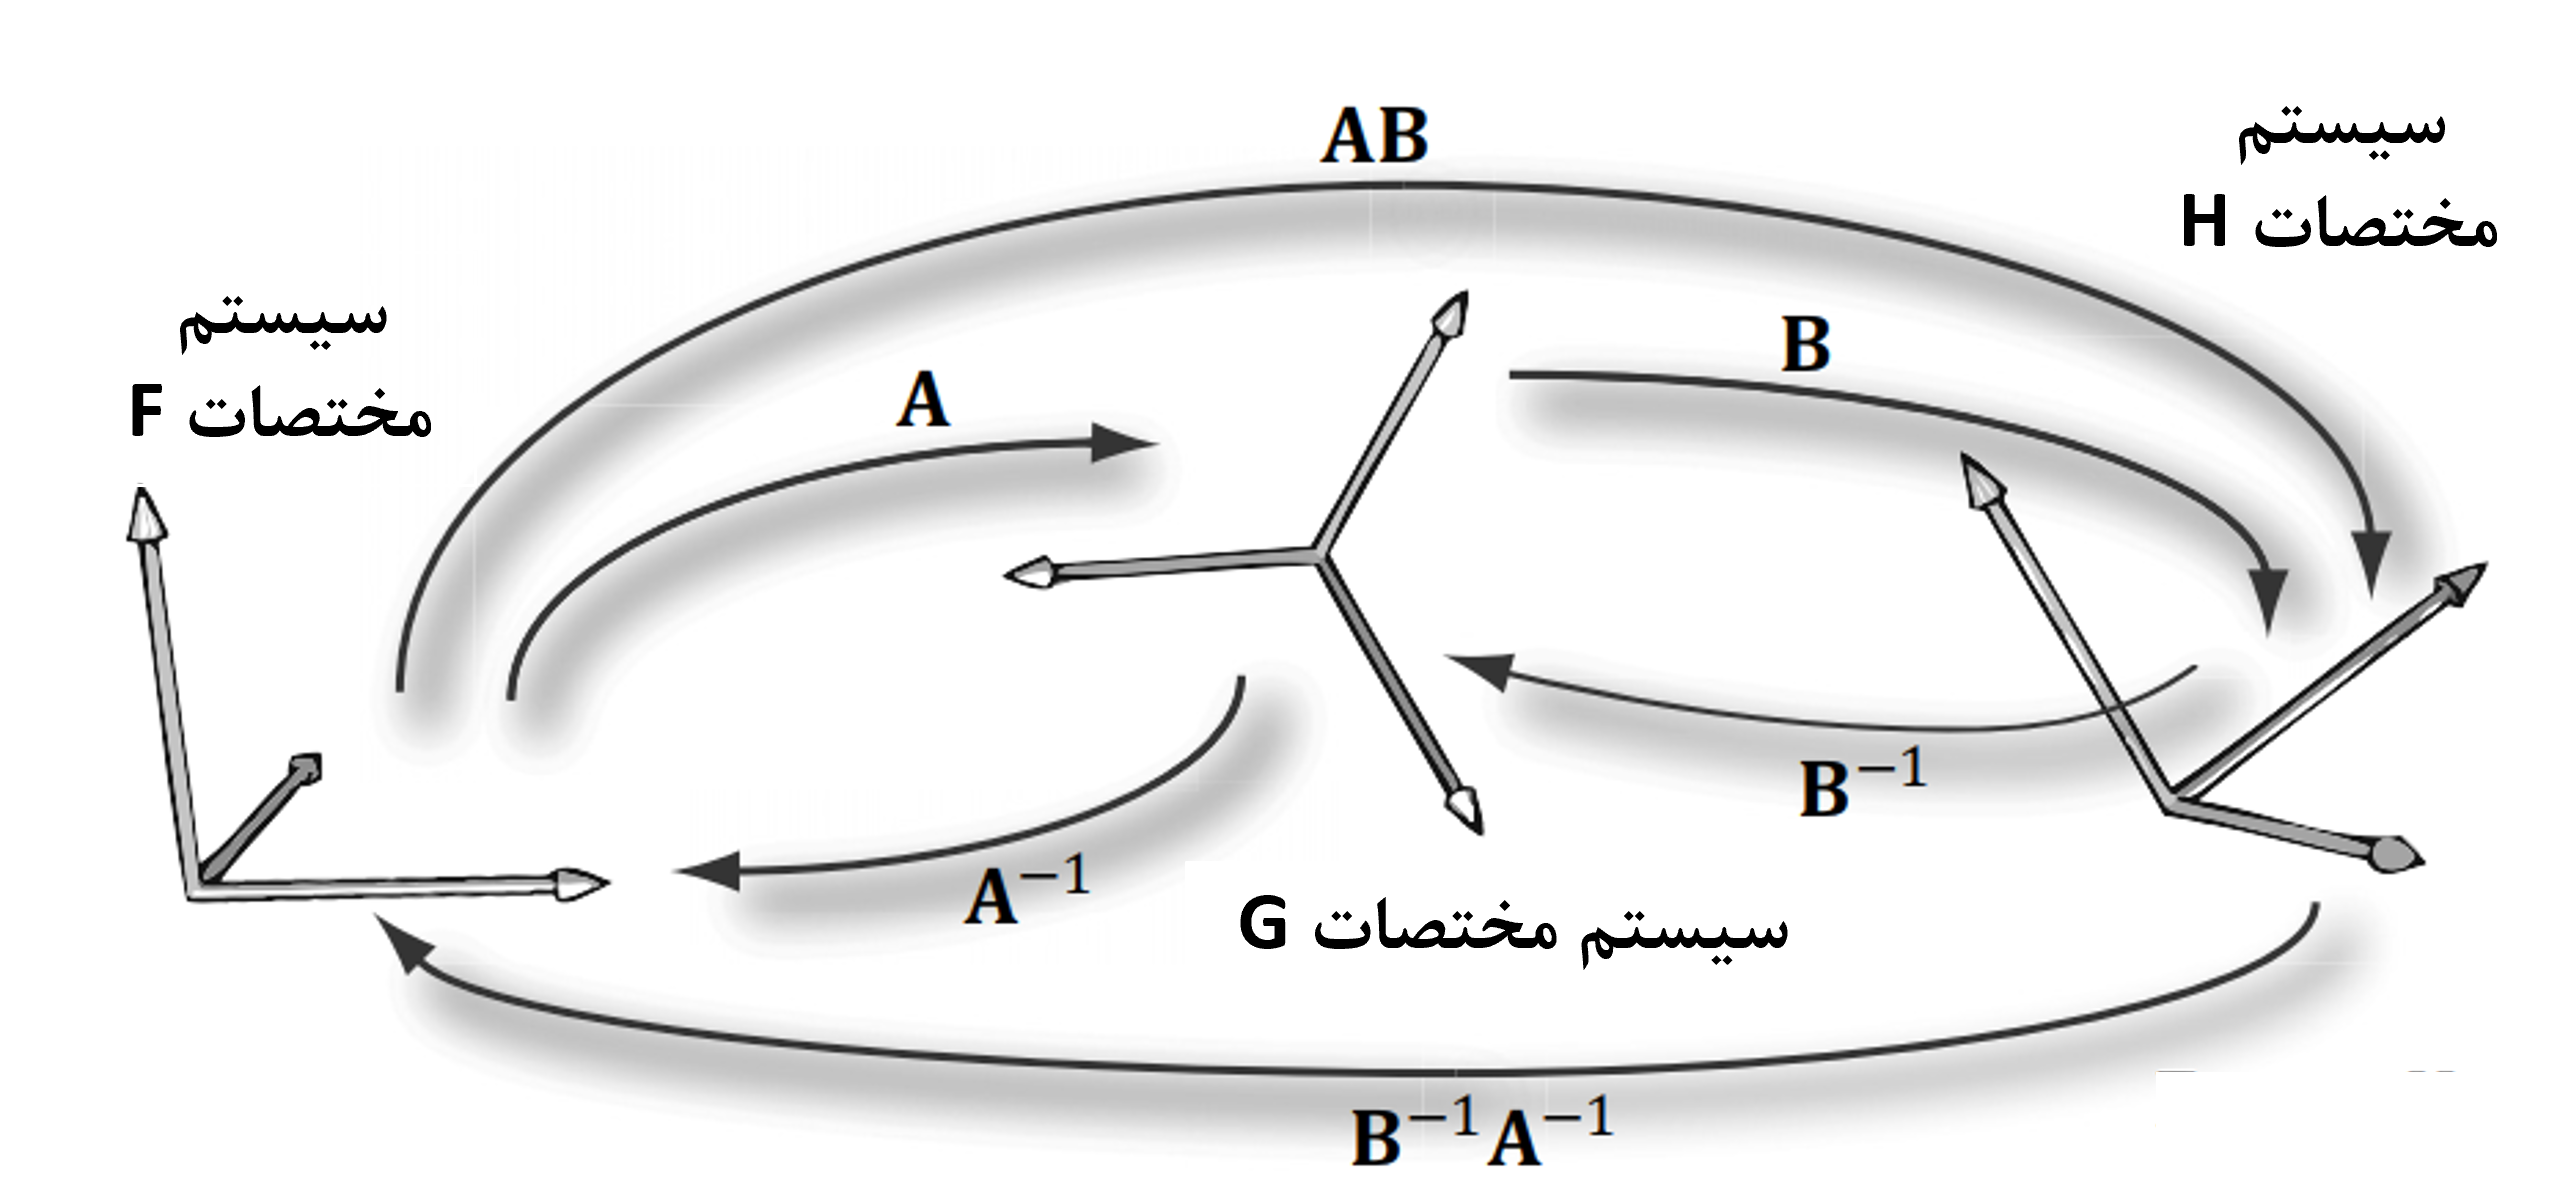
\includegraphics[width=0.8\textwidth]{Images/4/3/4.Session.1.3.14}
            \caption {نقشه های $\textbf{A}$ از $F$ به $G$، $\textbf{B}$ از $G$ به $H$، و $\textbf{AB}$ از $F$ به طور مستقیم به $H$ نقشه میکند. $\textbf{B}^{-1}$ از $H$ به $G$، $\textbf{A}^{-1}$ از $G$ به $F$ و $\textbf{B}^{-1}\textbf{A}^{-1}$ به طور مستقیم از $H$ به $F$ نقشه میکند.}
            \label{fig:4.Session.1.3.14}
        \end{figure}

    \end{spacing}
}

\subsection{\textbf{معکوس ها در مقابل تغییر ماتریس های مختصات}}
{
    \Large
    \begin{spacing}{1.5}
        تاکنون بین تبدیل‌های «فعال» (مقیاس‌بندی، دوران، انتقال) و تغییر تبدیل مختصات تمایز قائل شده‌ایم.
        در این بخش خواهیم دید که از نظر ریاضی، این دو معادل هستند، و یک تبدیل فعال را می توان به عنوان تغییر تبدیل مختصات تفسیر کرد، و برعکس.
        شکل \ref{fig:4.Session.1.3.15} شباهت هندسی بین ردیف ها را در معادله \ref{eqtn:3.7} نشان می دهد (دوران و به دنبال آن انتقال وابسته است. ماتریس تبدیل) و ردیف های معادله \ref{eqtn:3.9} (تغییر ماتریس مختصات).

        \begin{figure}[H]
            \centering
            \setlength{\belowcaptionskip}{-10pt}
            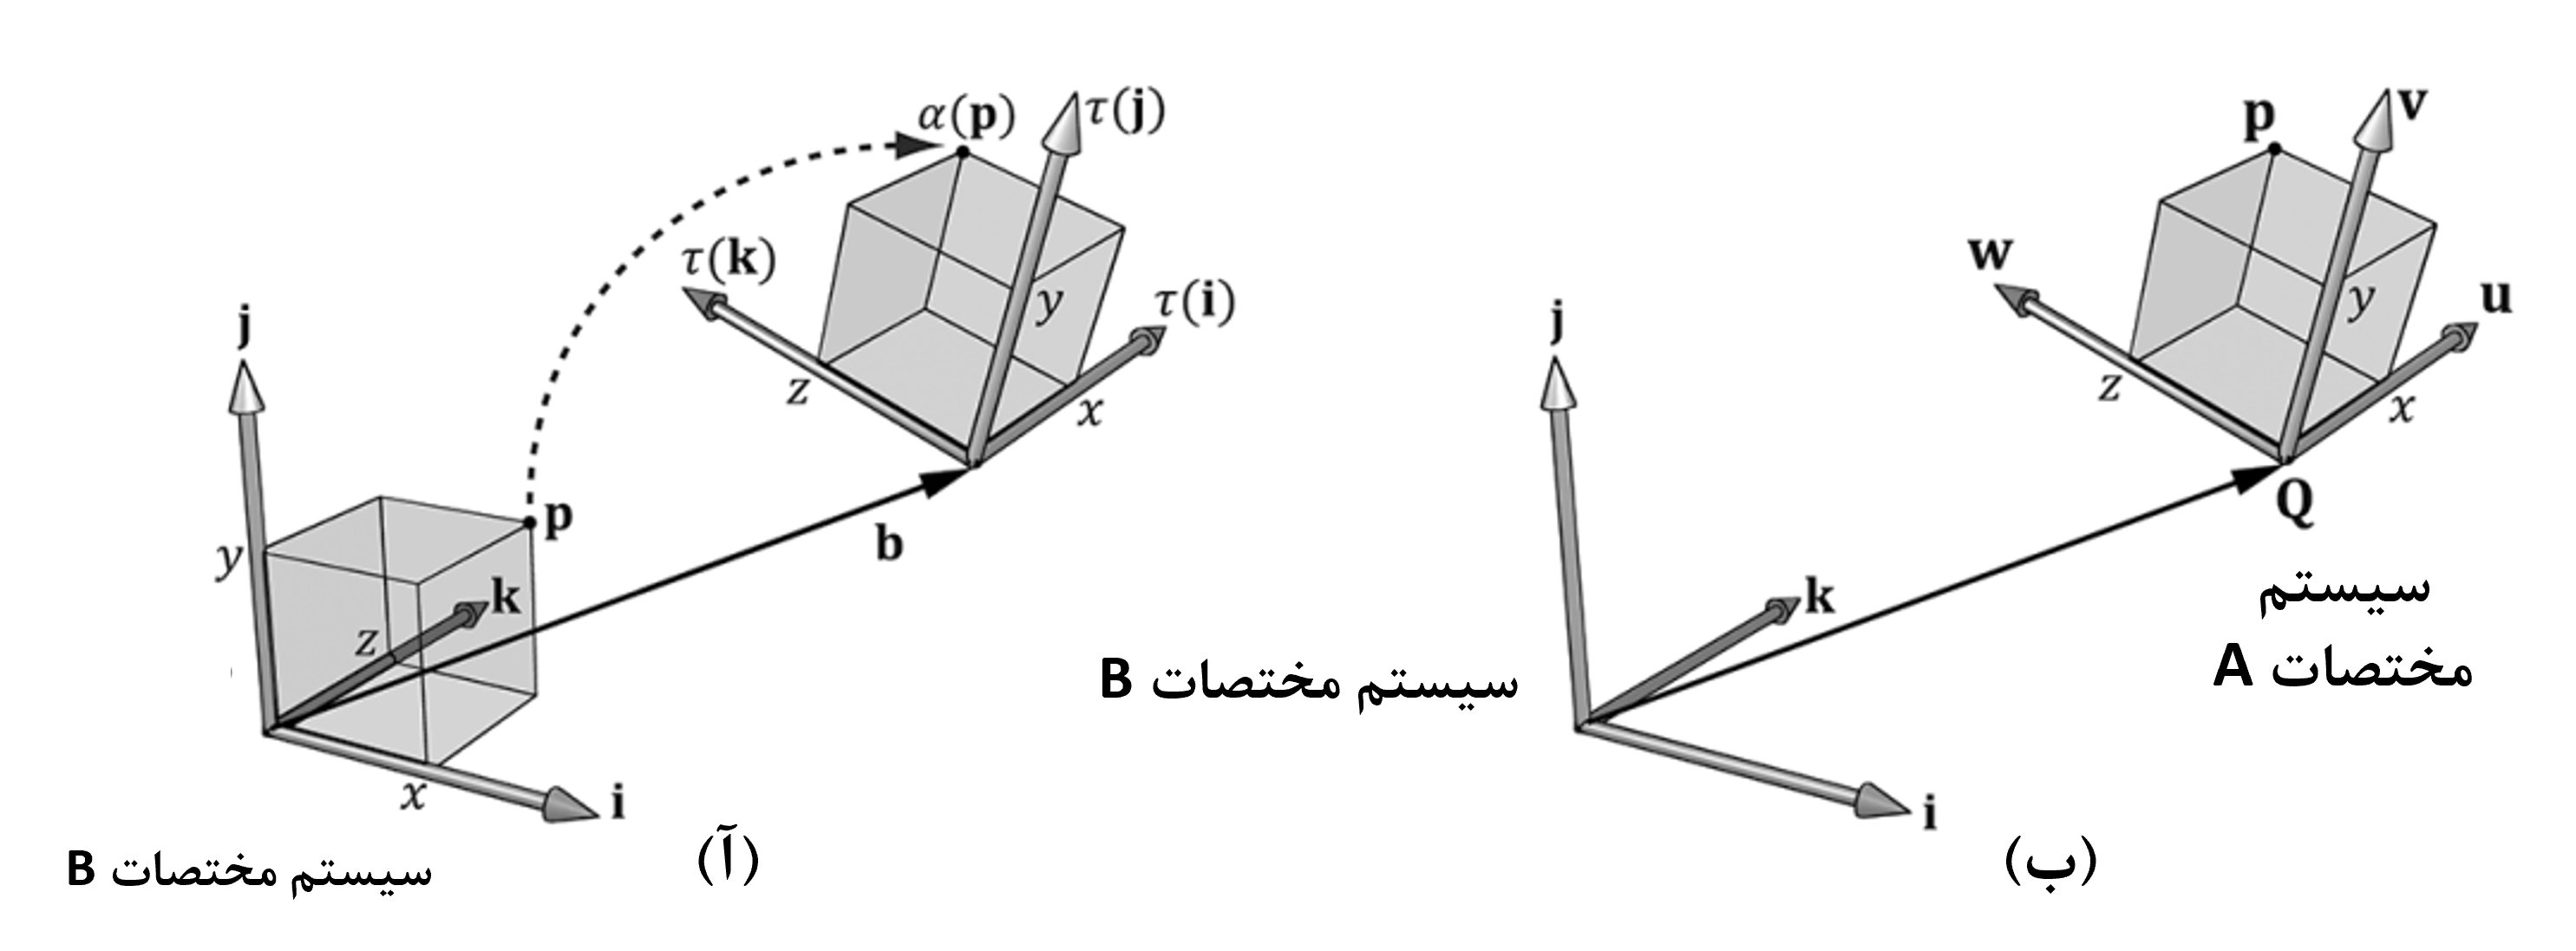
\includegraphics[width=0.5\textwidth]{Images/4/3/4.Session.1.3.15}
            \caption {می بینیم که$\textbf{b}=\textbf{Q}$،$\tau(\textbf{i})=\textbf{u}$، $\tau(\textbf{j})=\textbf{v}$ و $\tau(\textbf{k})=\textbf{w}$.
                (آ) ما با یک سیستم مختصات کار می کنیم، آن را سیستم مختصات $B$ می نامیم، و یک تبدیل آفینی به مکعب اعمال می کنیم
                تا موقعیت و جهت آن را نسبت به سیستم مختصات $B$ تغییر دهیم: $\alpha(x,y,z,w)=x\tau(\textbf{i})+y\tau(\textbf{j})+z\tau(\textbf{k})+w\textbf{b}$.
                (ب) ما دو سیستم مختصات به نام‌های سیستم مختصات $A$ و سیستم مختصات $B$ داریم.
                نقاط مکعب نسبت به سیستم مختصات $A$ را می‌توان با فرمول $\textbf{p}_{B}=x\textbf{u}_{B}+y\textbf{v}_{B}+z\textbf{w}_{B}+w\textbf{Q}_{B}$ به مختصات سیستم مختصات $B$ تبدیل کرد، که در آن $\textbf{p}_{A}=(x,y,z,w)$.
                در هر دو حالت، $\alpha(\textbf{p})=(x\prime,y\prime,z\prime,w)=\textbf{p}_{B}$ با مختصاتی نسبت به سیستم مختصات $B$ داریم.}
            \label{fig:4.Session.1.3.15}
        \end{figure}

        اگر به این فکر کنیم، منطقی است. زیرا با تغییر تبدیل مختصات، سیستم های مختصات در موقعیت و جهت متفاوت هستند.
        بنابراین، فرمول تبدیل ریاضی برای رفتن از یک سیستم مختصات به سیستم مختصات دیگر مستلزم دوران و انتقال مختصات است
        و بنابراین ما به همان شکل ریاضی می رسیم. در هر صورت، ما با اعداد یکسانی مواجه می شویم.
        تفاوت در نحوه تفسیر ما از تبدیل است. برای برخی موقعیت‌ها، کار با سیستم‌های مختصات متعدد و تبدیل بین سیستم‌هایی که شی بدون تغییر باقی می‌ماند، شهودی‌تر است،
        اما از آنجایی که نسبت به چارچوب مرجع متفاوتی توضیح داده می‌شود، نمایش مختصات آن تغییر می‌کند (این وضعیت با قسمت ب شکل \ref{fig:4.Session.1.3.15} مطابقت دارد. ).
        مواقع دیگر، ما می خواهیم یک شی را در داخل یک سیستم مختصات بدون تغییر چارچوب مرجع خود تبدیل کنیم (این وضعیت با قسمت الف شکل \ref{fig:4.Session.1.3.15} مطابقت دارد).

        \begin{point}{pnt:3.1}
            \Large
            به طور خاص، این بحث نشان می دهد که ما می توانیم ترکیبی از تبدیل های فعال (مقیاس بندی، دوران، انتقال) را به عنوان تغییر تبدیل مختصات تفسیر کنیم.
            این مهم است زیرا ما اغلب فضای جهانی خود را (فصل 5) تغییر ماتریس مختصات را به عنوان ترکیبی از تغییر مقیاس، دوران و انتقال تعریف می کنیم.
        \end{point}
    \end{spacing}
}


\section{\textbf{توابع تبدیل ریاضی \lr{DirectX}}}
\label{sec:3.5}
{
    \Large
    \begin{spacing}{1.5}
        ما توابع ریاضی تبدیل مرتبط با DirectX را برای مرجع خلاصه می کنیم.

        \textbf{\vspace{6pt}}
        \lr{\lstinputlisting[language=C++, firstline=50, lastline=95]{Codes/4.1.3.program.c}}
        \textbf{\vspace{6pt}}

        برای دو تابع آخر \texttt{XMVector3TransformCoord} و \texttt{XMVector3TransformNormal}، نیازی به تنظیم مختصات $w$ ندارید.
        توابع همیشه از $v_{w}=1$ و $v_{w}=0$ برای \texttt{XMVector3TransformCoord} و \texttt{XMVector3TransformNormal} استفاده به ترتیب می کنند.
    \end{spacing}
}
%-----------------------------------------------------------------------------------------------------------%
\newpage


\section{\textbf{خلاصه}}
\label{sec:3.6}
{
    \Large
    \begin{spacing}{1.5}
        \begin{enumerate}[label=\textbf{\arabic*}.]
            \item {ماتریس‌های بنیادی تبدیل - مقیاس‌بندی، دوران و انتقال - به صورت زیر هستند:
                $\textbf{S}=\begin{bmatrix}
                                s_x & 0   & 0   & 0 \\
                                0   & s_y & 0   & 0 \\
                                0   & 0   & s_z & 0 \\
                                0   & 0   & 0   & 1
                \end{bmatrix}\hspace{5 mm}\textbf{T}=\begin{bmatrix}
                                                         1     & 0     & 0     & 0 \\
                                                         0     & 1     & 0     & 0 \\
                                                         0     & 0     & 1     & 0 \\
                                                         b_{x} & b_{y} & b_{z} & 1
                \end{bmatrix}\hspace{5 mm}\textbf{R}_{n}=\begin{bmatrix}
                                                             c+(1-c)x^{2} & (1-c)xy+sz & (1-c)xz-sy & 0\\
                                                             (1-c)xy-sz & c+(1-c)y^{2} & (1-c)yz+sx & 0\\
                                                             (1-c)xz+sy & (1-c)yz-sx & c+(1-c)z^{2} & 0
                                                             0 & 0 & 0 & 1
                \end{bmatrix}$
            }

            \item {ما از ماتریس $4\times 4$ برای نشان دادن تبدیل ها و $1\times 4$ مختصات همگن برای توصیف نقاط و بردارها استفاده می کنیم،
            جایی که یک نقطه را با تنظیم جزء چهارم روی $w=1$ و یک بردار را با تنظیم $w=0$ نشان می دهیم.
            به این ترتیب، انتقال ها برای نقاط اعمال می شود اما برای بردارها اعمال نمی شود.}

            \item {یک ماتریس متعامد است اگر همه بردارهای ردیف آن واحد طول و متعامد باشند.
            یک ماتریس متعامد دارای خاصیت ویژه ای است که معکوس آن برابر با جابجایی آن است،
            در نتیجه محاسبه معکوس آسان و کارآمد می شود. همه ماتریس های چرخش متعامد هستند.}

            \item {از ویژگی تداعی ضرب ماتریس، می‌توانیم چندین ماتریس تبدیل را در یک ماتریس تبدیل ترکیب کنیم، که نشان‌دهنده اثر خالص اعمال متوالی ماتریس‌های جداگانه است.}

            \item {فرض کنید $\textbf{Q}_{B}$، $\textbf{u}_{B}$، $\textbf{v}_{B}$، و $\textbf{w}_{B}$ مبدا، محورهای $x$، $y$ و $z$ سیستم مختصات $A$ را با مختصاتی نسبت به سیستم مختصات $B$ به ترتیب توصیف کنند.
            اگر یک بردار/نقطه $\textbf{p}$ مختصات $\textbf{p}_{A}=(x,y,z)$ نسبت به سیستم مختصات $A$ داشته باشد، همان بردار/نقطه نسبت به سیستم مختصات $B$ مختصاتی دارد:
                \begin{flushleft}
                    \lr{$\textbf{p}_{B}=(x\prime,z\prime,y\prime)=x\textbf{u}_{B}+y\textbf{v}_{B}+z\textbf{w}_{B}$\hspace{19 mm} \rl{(برای بردارها (جهت و اندازه))}\\
                        $\textbf{p}_{B}=(x\prime,z\prime,y\prime)=\textbf{Q}_{B}+x\textbf{u}_{B}+y\textbf{v}_{B}+z\textbf{w}_{B}$\hspace{35 mm} \rl{(برای بردارهای موقعیت (نقاط))}
                    }
                \end{flushleft}
                این تغییر تبدیل مختصات را می توان بر حسب ماتریس با استفاده از مختصات همگن نوشت.
            }

            \item {فرض کنید سه سیستم مختصات داریم، $F$، $G$ و $H$، و اجازه دهید $\textbf{A}$ تغییر ماتریس سیستم مختصات از $F$ به $G$ باشد، و اجازه دهید $\textbf{A}$ تغییر ماتریس سیستم مختصات از $G$ به $H$ باشد.
            با استفاده از ضرب ماتریس-ماتریس، ماتریس $\textbf{C}=\textbf{AB}$ را می توان به عنوان تغییر ماتریس سیستم مختصات $F$ به طور مستقیم به $H$ در نظر گرفت.
            یعنی ضرب ماتریس-ماتریس اثرات $\textbf{A}$ و $\textbf{B}$ را در یک ماتریس خالص ترکیب می کند و بنابراین می توانیم بنویسیم:
                $\textbf{p}_{F}(\textbf{AB})=\textbf{p}_{H}$}

            \item {اگر ماتریس $\textbf{M}$ مختصات سیستم مختصات $A$ را در مختصات سیستم مختصات $B$ ترسیم کند،
            ماتریس $\textbf{M}^{-1}$ مختصات سیستم مختصات $B$ را در مختصات سیستم مختصات $A$ ترسیم می کند.}

            \item {یک تبدیل فعال را می توان به عنوان تغییر تبدیل مختصات تفسیر کرد و برعکس.
            برای برخی موقعیت‌ها، کار با سیستم‌های مختصات متعدد و تبدیل بین سیستم‌هایی که شی بدون تغییر باقی می‌ماند، شهودی‌تر است،
            اما از آنجایی که نسبت به چارچوب مرجع متفاوتی توصیف می‌شود، نمایش مختصات آن تغییر می‌کند.
            مواقع دیگر، ما می خواهیم یک شی را در داخل یک سیستم مختصات بدون تغییر چارچوب مرجع خود تبدیل کنیم.}
        \end{enumerate}
    \end{spacing}
}
%-----------------------------------------------------------------------------------------------------------%
\newpage


\section{\textbf{تمارین}}
\label{sec:3.7}
{
    \Large
    \begin{spacing}{1.5}
        \begin{enumerate}[label=\textbf{\arabic*}.]
            \item {فرض کنید $\tau: \mathbb{R}^3\rightarrow\mathbb{R}^3$ با $\tau(x,y,z)=(x+y,x-3,z)$ تعریف شود.
            آیا $\tau$ تبدیل خطی است؟ اگر چنین است، نمایش ماتریس استاندارد آن را پیدا کنید.}

            \item {فرض کنید $\tau: \mathbb{R}^3\rightarrow\mathbb{R}^3$ با $\tau(x,y,z)=(3x+4z, 2x–z, x+y+z)$ تعریف شود.
            آیا $\tau$ تبدیل خطی است؟ اگر چنین است، نمایش ماتریس استاندارد آن را پیدا کنید.}

            \item {فرض کنید $\tau: \mathbb{R}^3\rightarrow\mathbb{R}^3$ تبدیل خطی است.
            بعلاوه فرض کنید که $\tau(1,0,0)=(3,1,1)$، $\tau(0,1,0)=(2,-1,3)$ و $\tau(0,0,1)=(4,0,2)$. $\tau(1,1,1)$ را پیدا کنید.}

            \item {یک ماتریس مقیاس‌بندی بسازید که در محور $x$ $2$ واحد، در محور $y$ $-3$ واحد باشد و بعد $z$ را بدون تغییر نگه دارد.}

            \item {یک ماتریس دوران بسازید که 30 درجه در امتداد محور $(1,1,1)$ دوران کند.}

            \item {یک ماتریس انتقال بسازید که $4$ واحد در محور $x$، صفر واحد در محور $y$ و $9$ واحد در محور $z$ انتقال یابد.}

            \item {یک ماتریس تبدیل واحد بسازید که ابتدا $2$ واحد در محور $x$، $-3$ واحد در محور $y$، و بعد $z$ را بدون تغییر نگه دارد، و سپس $4$ واحد را در محور $x$ انتقال یابد، صفر واحد در محور $y$، و $-9$ واحد در محور $z$.}

            \item {یک ماتریس تبدیل واحد بسازید که ابتدا $45$ درجه حول محور $y$ دوران کند و سپس $2$ واحد در محور $x$، $5$ واحد در محور $y$ و $1$ واحد در محور $z$ انتقال یابد.}

            \item {مثال \ref{exp:3.2} را دوباره انجام دهید، اما این بار مربع را $1.5$ واحد در محور $x$، $0.75$ واحد در محور $y$، و محور $z$ را بدون تغییر رها کنید.
            شکل هندسی را قبل و بعد از تبدیل ترسیم کنید تا درستی کار خود را بررسی کنید.}

            \item {مثال \ref{exp:3.3} را دوباره انجام دهید، اما این بار مربع را $45-$ درجه در جهت عقربه های ساعت حول محور $y$ بچرخانید (یعنی $45$ درجه خلاف جهت عقربه های ساعت).
            شکل هندسی را قبل و بعد از تبدیل ترسیم کنید تا درستی کار خود را بررسی کنید.}

            \item {مثال \ref{exp:3.4} را دوباره انجام دهید، اما این بار مربع $-5$ واحد در محور $x$، $-3.0$ واحد در محور $y$ و $4.0$ واحد در محور $z$ انتقال دهید.
            شکل هندسی را قبل و بعد از تبدیل ترسیم کنید تا درستی کار خود را بررسی کنید.}

            \item {نشان دهید که $R_{n}(\textbf{v})=\cos\theta\textbf{v}+(1-\cos\theta)(\textbf{n}\cdot\textbf{v})\textbf{n}+\sin\theta(\textbf{n}\times\textbf{v})$ یک تبدیل خطی است و نمایش ماتریس استاندارد آن را پیدا کنید.}

            \item {ثابت کنید که ردیف های $\textbf{R}_{y}$ متعامد هستند. برای تمرین محاسباتی فشرده تر، خواننده می تواند این کار را برای ماتریس دوران عمومی (ماتریس دوران حول یک محور دلخواه) نیز انجام دهد.}

            \item {ثابت کنید که ماتریس $\textbf{M}$ متعامد است اگر و تنها اگر$\textbf{M}^{T}=\textbf{M}^{-1}$ باشد.}

            \item { محاسبه کنید:
                \begin{center}
                    $[x, y, z, 1]\begin{bmatrix}
                                     1 & 0 & 0 & 0 \\
                                     0 & 1 & 0 & 0 \\
                                     0 & 0 & 1 & 0
                                     b_{x} & b_{y} & b_{y} & 1
                    \end{bmatrix}=[x\prime, y\prime, z\prime,1]$ \hspace{5 mm}
                    $[x, y, z, 0]\begin{bmatrix}
                                     1 & 0 & 0 & 0 \\
                                     0 & 1 & 0 & 0 \\
                                     0 & 0 & 1 & 0
                                     b_{x} & b_{y} & b_{y} & 1
                    \end{bmatrix}=[x\prime, y\prime, z\prime,1]$
                \end{center}
                آیا انتقال نقاط را منتقل می کند؟ آیا انتقال بردارها را منتقل می کند؟ چرا انتقال مختصات یک بردار در موقعیت استاندارد منطقی نیست؟
            }

            \item {بررسی کنید که معکوس ماتریس مقیاس بندی داده شده در واقع معکوس ماتریس مقیاس بندی است.
            یعنی با انجام مستقیم ضرب ماتریس، $\textbf{SS}^{-1}=\textbf{S}^{-1}\textbf{S}=\textbf{I}$ را نشان دهید. یعنی نشان دهید که $\textbf{TT}^{-1}=\textbf{T}^{-1}\textbf{T}=\textbf{I}$.}

            \item {فرض کنید که سیستم های مختصات $A$ و $B$ را داریم.
            فرض کنید $\textbf{p}_{A}=(1,-2,0)$ و$\textbf{q}_{A}=(1,2,0)$ به ترتیب یک نقطه و نیرو را نسبت به سیستم مختصات $A$ نشان میدهند.
            علاوه بر این، فرض کنید$\textbf{Q}_{B}=(-6,2,0)$، $\textbf{u}_{B}=\left(\frac{\displaystyle 1}{\sqrt{\displaystyle 2}},\frac{\displaystyle 1}{\sqrt{\displaystyle 2}},0 \right)$، $\textbf{v}_{B}=\left(\frac{\displaystyle -1}{\sqrt{\displaystyle 2}},\frac{\displaystyle 1}{\sqrt{\displaystyle 2}},0 \right)$ و $\textbf{w}_{B}=(0,0,1)$ با مختصات $A$ به سیستم مختصات $B$ را توصیف می کنند.
            تغییر ماتریس مختصات را بسازید که مختصات سیستم مختصات $A$ را به مختصات سیستم مختصات $B$ ترسیم می کند و $\textbf{p}_{B}=(x,y,z)$ و $\textbf{q}_{B}=(x,y,z)$ را پیدا کنید.
            یک تصویر روی کاغذ گراف بکشید تا مطمئن شوید که پاسخ شما منطقی است.}

            \item {
                آنالوگ نقاط به ترکیب خطی بردارها یک ترکیب آفین است:
                $\textbf{p}=a_{1}\textbf{p}_{1}+\dots+a_{n}\textbf{p}_{n}$ که در آن $a_{1}+\dots+a_{n}=1$ و $p_{1}+\dots+p_{n}$ نقاط هستند.
                ضریب اسکالر $a_{k}$ را می توان به عنوان وزن "نقطه ای" در نظر گرفت
                که نشان می دهد نقطه $\textbf{p}_{k}$ چقدر در تعیین $\textbf{p}$ تأثیر دارد.
                به زبان ساده، هر چه $a_{k}$ به $1$ نزدیکتر باشد،
                $\textbf{p}$ به $\textbf{p}_{k}$ نزدیکتر خواهد بود و $\textbf{p}_{k}$ منفی، $\textbf{p}$ را از $\textbf{p}_{k}$ «دفع» می کند.
                (تمرین بعدی به شما کمک می کند تا حدی شهود در این مورد ایجاد کنید.) وزن ها به نام مختصات باریکانسریک نیز شناخته می شوند.
                نشان دهید که یک ترکیب آفین را می توان به عنوان یک نقطه به اضافه یک بردار نوشت:
                \begin{center}
                    $\textbf{p}=\textbf{p}_{1}+a_{2}(\textbf{p}_{2}-\textbf{p}_{1})+\dots+a_{n}(\textbf{p}_{n}-\textbf{p}_{1})$
                \end{center}
            }

            \item {
                مثلثی را که با نقاط $\textbf{p}_{1}=(0,0,0)$، $\textbf{p}_{2}=(0,1,0)$ و $\textbf{p}_{3}=(2,0,0)$ تعریف شده است، در نظر بگیرید. نقاط زیر را نمودار کنید:
                \lr{
                    \begin{flushleft}
                    (a)
                        $\frac{\displaystyle 1}{\displaystyle 3}\textbf{p}_{1}+\frac{\displaystyle 1}{\displaystyle 3}\textbf{p}_{2}+\frac{\displaystyle 1}{\displaystyle 3}\textbf{p}_{3}$ \\
                        (b) $0.7\textbf{p}_{1}+0.2\textbf{p}_{2}+0.1\textbf{p}_{3}$ \\
                        (c) $0.0\textbf{p}_{1}+0.5\textbf{p}_{2}+0.5\textbf{p}_{3}$ \\
                        (d) $-0.2\textbf{p}_{1}+0.6\textbf{p}_{2}+0.6\textbf{p}_{3}$ \\
                        (e) $0.6\textbf{p}_{1}+0.5\textbf{p}_{2}-0.1\textbf{p}_{3}$ \\
                        (f) $0.8\textbf{p}_{1}-0.3\textbf{p}_{2}+0.5\textbf{p}_{3}$ \\
                    \end{flushleft}
                    نقطه در قسمت (\lr{a}) چیست؟ مختصات باریسنتریک $\textbf{p}_{2}$ و نقطه $(1,0,0)$ بر حسب $\textbf{p}_{1}$، $\textbf{p}_{2}$ و ​​$\textbf{p}_{3}$ چه خواهد بود؟ آیا می توانید حدس بزنید که اگر یکی از مختصات باری مرکزی منفی باشد، نقطه $\textbf{p}$ نسبت به مثلث در کجا قرار می گیرد؟
                } \textbf{\vspace{-6pt}}
            }

            \item {یکی از عوامل تعیین کننده تبدیل آفین این است که ترکیبات آفین را حفظ می کند.
            ثابت کنید که تبدیل آفین $\alpha(\textbf{u})$ تبدیل های آفین را حفظ می کند.
            یعنی $\alpha(a_{1}\textbf{p}_{1}+...+a_{n}\textbf{p}_{n})=a_{1}\alpha(\textbf{p}_{1})+...+a_{n}\alpha(\textbf{p}_{n})$ که در آن $a_{1}+...+a_{n}=1$.}

            \item {
                شکل \ref{fig:4.Session.1.3.16} را در نظر بگیرید.
                یک تغییر متداول تبدیل مختصات در گرافیک کامپیوتری این است که مختصات را از سیستم مختصات $A$ (مربع $[-1,1]^{2}$) به سیستم مختصات B (مربع $[0,1]^{2}$ که در آن محورهای $y$ در مقابل آن قرار می‌گیرند) نگاشت می‌کند. سیستم مختصات A).
                ثابت کنید که تغییر تبدیل مختصات را از سیستم مختصات $A$ به سیستم مختصات $B$ به وسیله:

                \begin{center}
                    $[x, y, 0, 1]\begin{bmatrix}
                                     0.5 & 0 & 0 & 0 \\
                                     0 & -0.5 & 0 & 0 \\
                                     0 & 0 & 1 & 0
                                     0.5 & 0.5 & 0 & 1
                    \end{bmatrix}=[x\prime, y\prime, 0, 1]$
                \end{center}

                \begin{figure}[H]
                    \centering
                    \setlength{\belowcaptionskip}{-10pt}
                    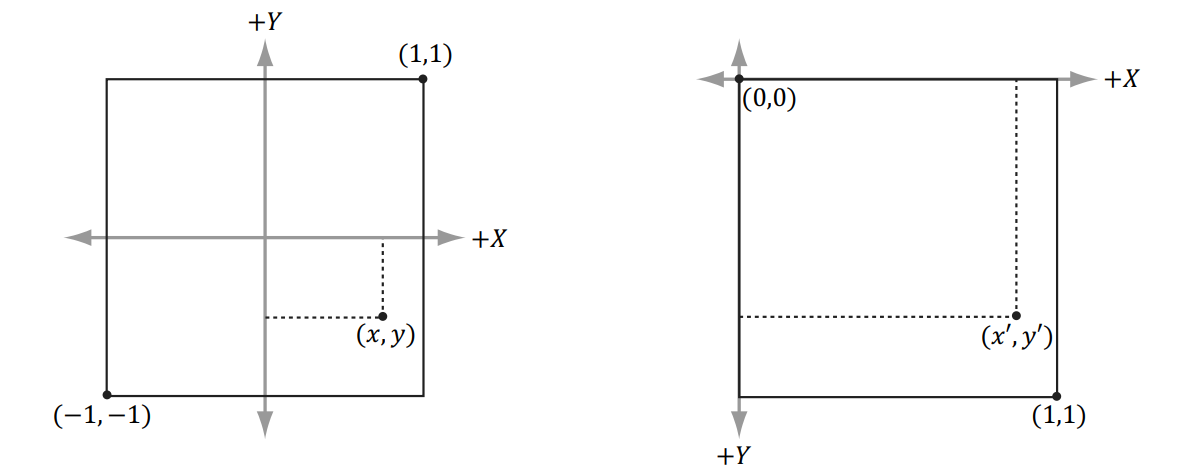
\includegraphics[width=0.8\textwidth]{Images/4/3/4.Session.1.3.16}
                    \caption {تغییر مختصات از سیستم مختصات $A$ (مربع $[-1,1]^{2}$) به سیستم مختصات B (مربع $[0,1]^{2}$ که در آن محورهای $y$ مخالف با سیستم مختصات $A$ هستند)}
                    \label{fig:4.Session.1.3.16}
                \end{figure}
            }

            \item {در فصل آخر ذکر شد که دترمینان مربوط به تغییر حجم یک جعبه تحت یک تبدیل خطی است.
            دترمینان ماتریس مقیاس بندی را پیدا کنید و نتیجه را بر حسب حجم تفسیر کنید.}

            \item {
                تبدیل $\tau$ را در نظر بگیرید که مربع را به متوازی الاضلاع تبدیل می کند:

                \begin{center}
                    $\tau(x,y)=(3x+y,x+2y)$
                \end{center}

                نمایش ماتریس استاندارد این تبدیل را بیابید و نشان دهید که دترمینان ماتریس تبدیل برابر است با مساحت متوازی الاضلاع که توسط $\tau(\textbf{i})$ و $\tau(\textbf{j})$ پوشانده شده است.

                \begin{figure}[H]
                    \centering
                    \setlength{\belowcaptionskip}{-10pt}
                    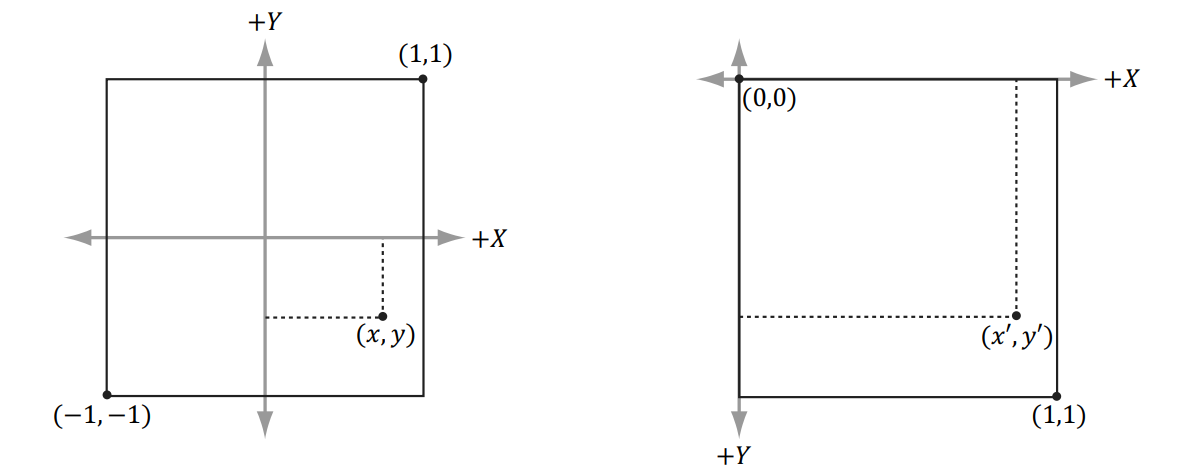
\includegraphics[width=0.8\textwidth]{Images/4/3/4.Session.1.3.16}
                    \caption {تبدیلی که مربع را به متوازی الاضلاع ترسیم می کند.}
                    \label{fig:4.Session.1.3.16}
                \end{figure}
            }

            \item {نشان دهید که دترمینان ماتریس دوران محور $y$، $1$ است. بر اساس تمرین بالا، توضیح دهید که چرا منطقی است که $1$ است.
            برای تمرین محاسباتی فشرده تر، خواننده می تواند دترمینان ماتریس دوران عمومی (دوران ماتریس حول یک محور دلخواه) را نشان دهد برابر 1 است.}

            \item {یک ماتریس دوران را می توان از نظر جبری به عنوان یک ماتریس متعامد با دترمینان برابر با $1$ مشخص کرد. بردارهای پایه دوران $\tau(\textbf{i})$، $\tau(\textbf{j})$، و $\tau(\textbf{k})$ واحد طول و متعامد هستند.
            علاوه بر این، nوران اندازه جسم را تغییر نمی دهد، بنابراین دترمینان باید $1$ باشد.
            نشان دهید که حاصل ضرب دو ماتریس دورانی $\textbf{R}_{1}\textbf{R}_{2}=\textbf{R}$ یک ماتریس دورانی است.
            یعنی $\textbf{RR}^{T}=\textbf{R}^{T}\textbf{R}=\textbf{I}$ را نشان دهید (برای نشان دادن متعامد بودن $\textbf{R}$) و $det\textbf{R}=1$ را نشان دهید.}

            \item {
                نشان دهید که خواص زیر برای یک ماتریس دورانی $\textbf{R}$ برقرار است و توضیح دهید که چرا همه این ویژگی ها برای تبدیل دورانی معنا دارند.
                \lr{
                    \begin{flushleft}
                    (a)
                        $\textbf{uR}\cdot\textbf{vR}=\textbf{u}\cdot\textbf{v}$\hspace{19 mm} \rl{حفظ ضرب داخلی} \\
                        (b) $\norm{\textbf{uR}}=\norm{\textbf{u}}$\hspace{19 mm} \rl{حفظ اندازه} \\
                        (c) $\theta(\textbf{uR},\textbf{vR})=\theta(\textbf{u},\textbf{v})$ \hspace{19 mm} \rl{حفظ زاویه، که در آن $\theta(x,y)$ به زاویه بین $\textbf{x}$ و $\textbf{y}$ ارزیابی می کند: $\theta(\textbf{x},\textbf{x})=\cos^{-1}\frac{\displaystyle x\cdot y}{\displaystyle \norm{x}\norm{y}}$}
                    \end{flushleft}
                    \begin{center}
                    \end{center}
                } \textbf{\vspace{-6pt}}
            }

            \item {یک ماتریس مقیاس بندی، دوران و انتقال پیدا کنید که حاصلضرب آن پاره خط را با نقطه شروع $\textbf{p}=(0,0,0)$ و نقطه پایانی $\textbf{q}=(0,0,1)$ به پاره خط با طول $2$ موازی با بردار تبدیل کند.$(1,1,1)$، با نقطه شروع $(3,1,2)$.}

            \item {
                فرض کنید جعبه ای داریم که در $(x,y,z)$ قرار دارد. تبدیل مقیاس‌بندی که ما تعریف کرده‌ایم از مبدا به‌عنوان نقطه مرجع برای مقیاس‌بندی استفاده می‌کند،
                بنابراین مقیاس‌بندی این کادر (نه در مرکز مبدا) اثر جانبی انتقال جعبه را دارد (شکل \ref{fig:4.Session.1.3.18}).
                این می تواند در برخی شرایط نامطلوب باشد. تبدیلی را پیدا کنید که کادر را نسبت به نقطه مرکزی آن مقیاس کند.

                \begin{hint}{hnt:2.1}
                    \Large
                    مختصات را به سیستم مختصات جعبه با مبدا در مرکز جعبه تغییر دهید، کادر را مقیاس کنید، سپس به سیستم مختصات اصلی تبدیل کنید.
                \end{hint} \\

                \begin{figure}[H]
                    \centering
                    \setlength{\belowcaptionskip}{-10pt}
                    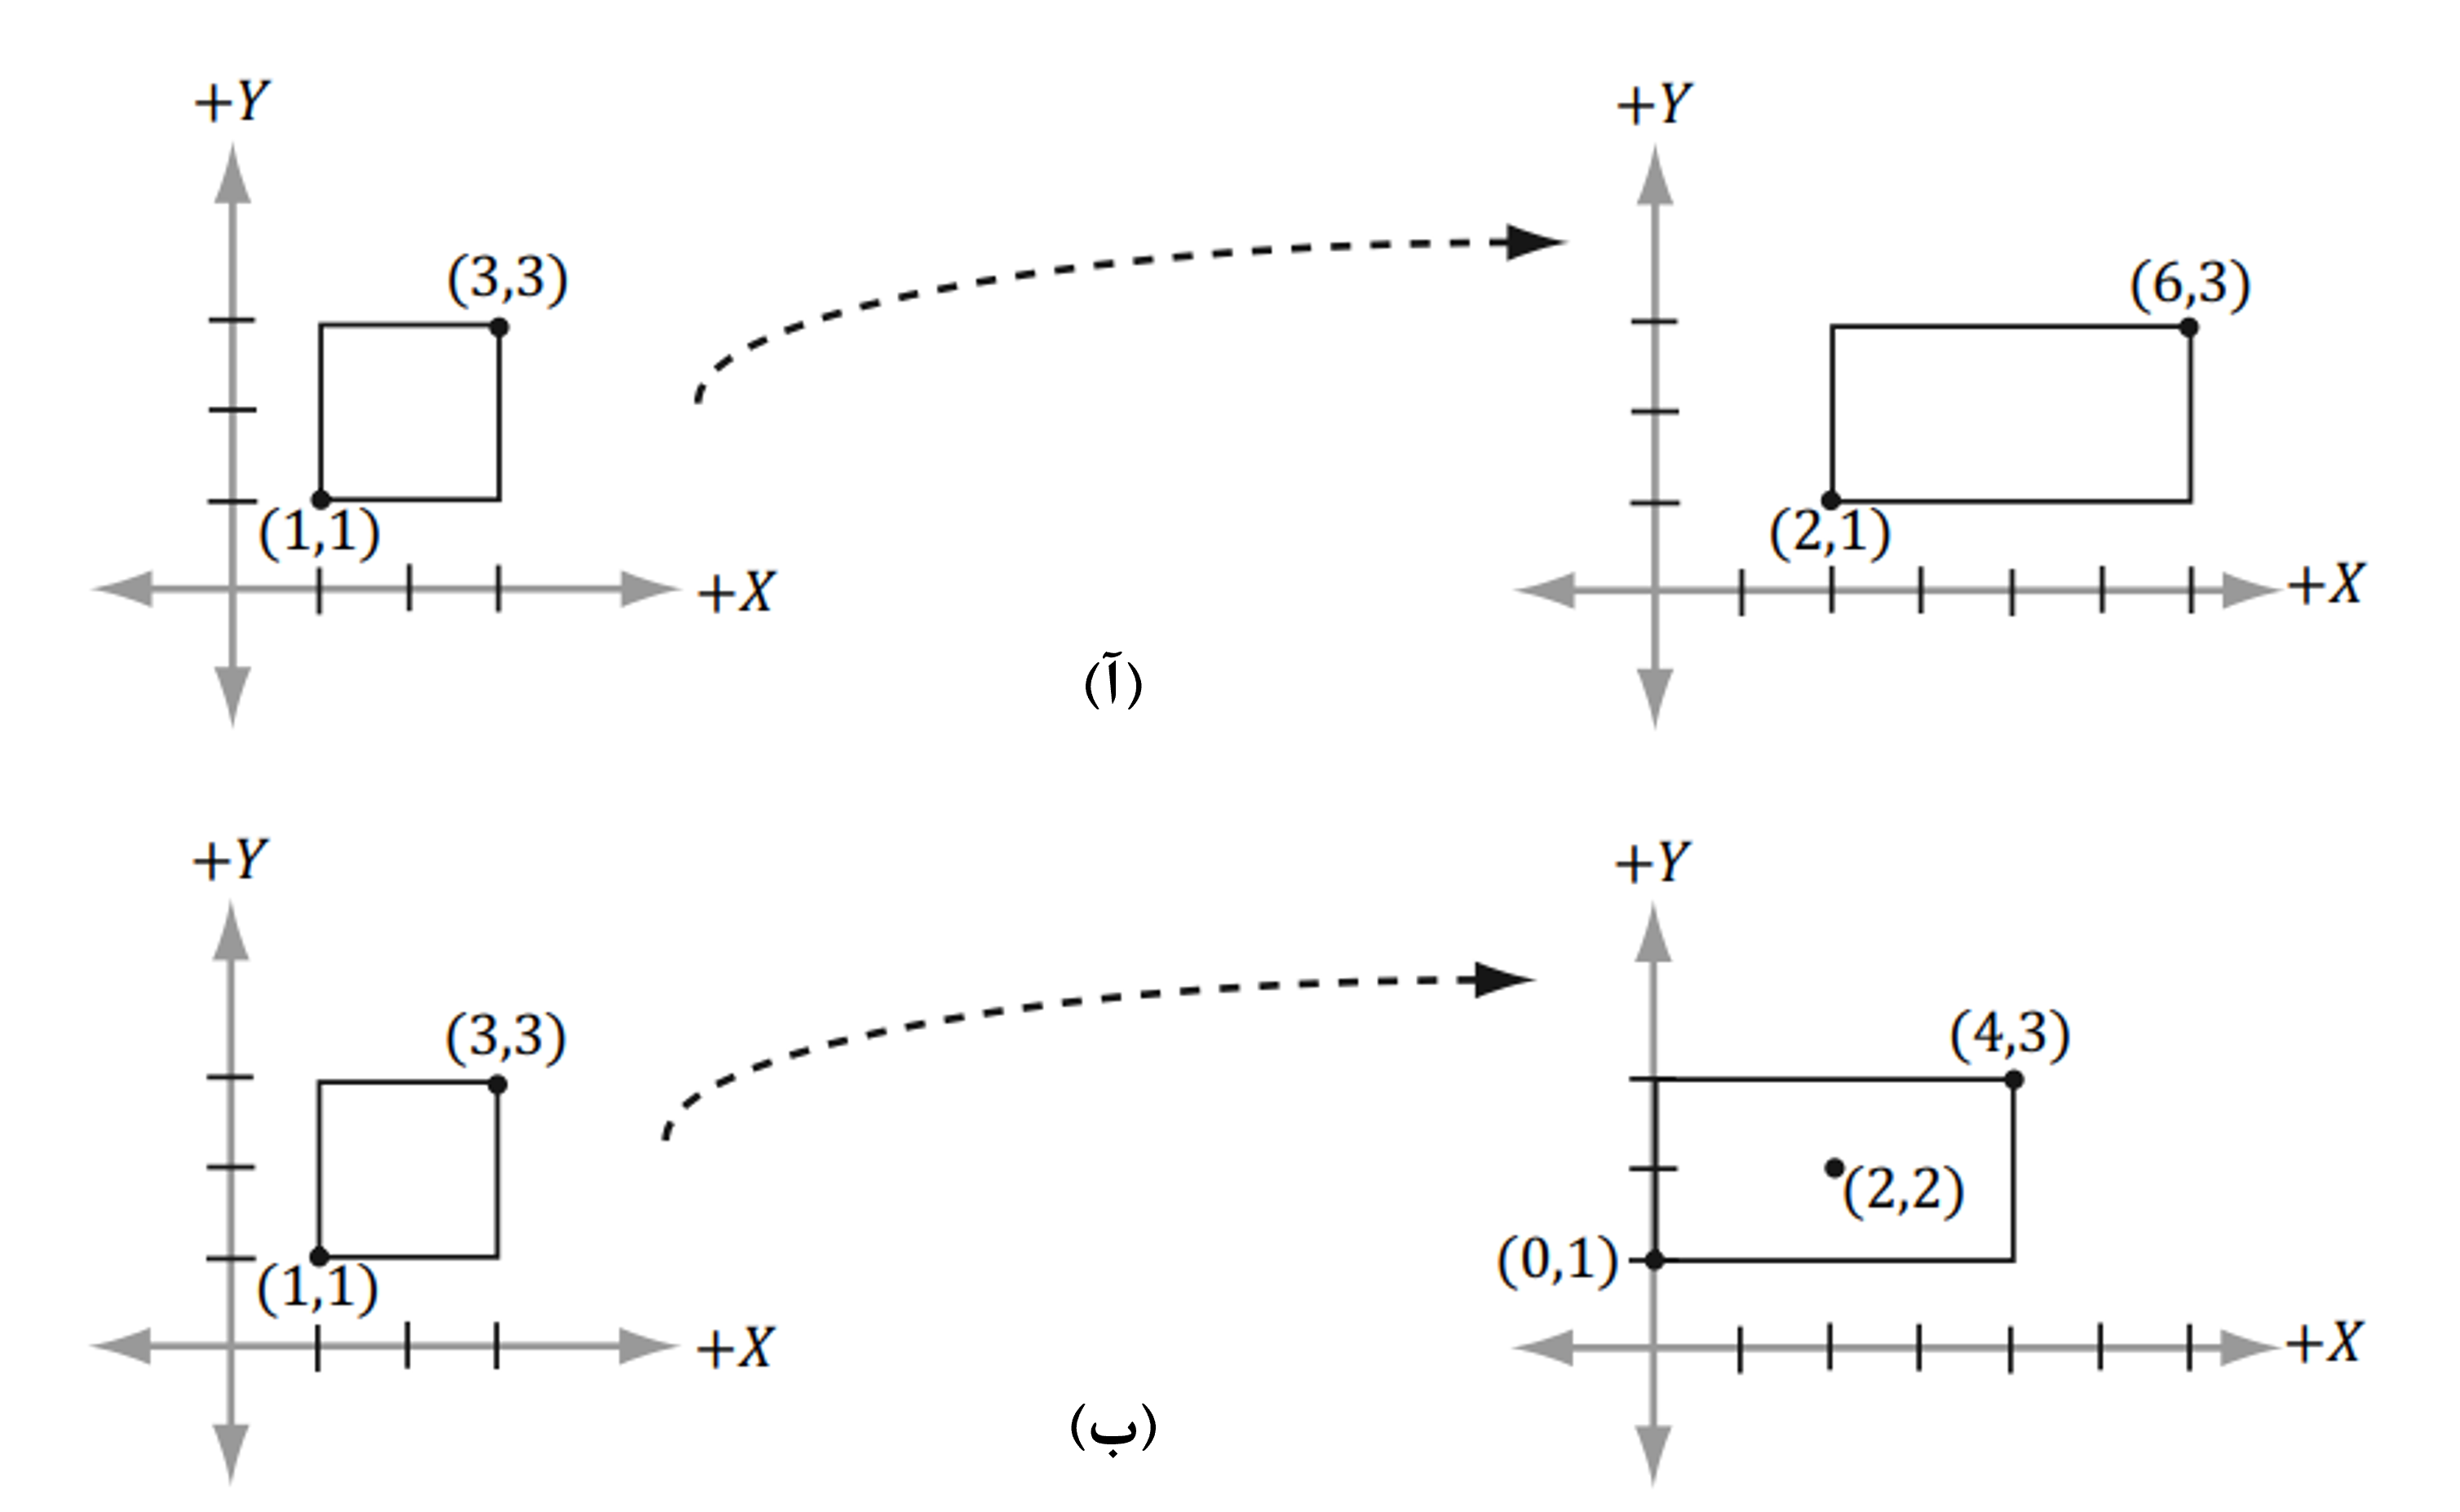
\includegraphics[width=0.8\textwidth]{Images/4/3/4.Session.1.3.18}
                    \caption {(آ) مقیاس $2$ واحد در محور $x$ نسبت به مبدا منجر به انتقال مستطیل می شود.
(ب) مقیاس $2$ واحد در محور $x$ نسبت به مرکز مستطیل منجر به انتقال نمی شود (مستطیل نقطه مرکزی اصلی خود را حفظ می کند).}
                    \label{fig:4.Session.1.3.18}
                \end{figure}
            }
        \end{enumerate}
    \end{spacing}
}